% Copyright (C) 2014-2015 by Thomas Auzinger <thomas@auzinger.name>

\documentclass[draft,final]{vutinfth} % Remove option 'final' to obtain debug information.

% Load packages to allow in- and output of non-ASCII characters.
\usepackage{lmodern}        % Use an extension of the original Computer Modern font to minimize the use of bitmapped letters.
\usepackage[T1]{fontenc}    % Determines font encoding of the output. Font packages have to be included before this line.
\usepackage[utf8]{inputenc} % Determines encoding of the input. All input files have to use UTF8 encoding.

% Extended LaTeX functionality is enables by including packages with \usepackage{...}.
\usepackage{fixltx2e}   % Provides fixes for several errors in LaTeX2e.
\usepackage{amsmath}    % Extended typesetting of mathematical expression.
\usepackage{amssymb}    % Provides a multitude of mathematical symbols.
\usepackage{mathtools}  % Further extensions of mathematical typesetting.
\usepackage{microtype}  % Small-scale typographic enhancements.
\usepackage{enumitem}   % User control over the layout of lists (itemize, enumerate, description).
\usepackage{multirow}   % Allows table elements to span several rows.
\usepackage{booktabs}   % Improves the typesettings of tables.
\usepackage{subcaption} % Allows the use of subfigures and enables their referencing.
\usepackage[ruled,linesnumbered,algochapter]{algorithm2e} % Enables the writing of pseudo code.
\usepackage[usenames,dvipsnames,table]{xcolor} % Allows the definition and use of colors. This package has to be included before tikz.
\usepackage{nag}       % Issues warnings when best practices in writing LaTeX documents are violated.
\usepackage{hyperref}  % Enables cross linking in the electronic document version. This package has to be included second to last.
\usepackage[acronym,toc]{glossaries} % Enables the generation of glossaries and lists fo acronyms. This package has to be included last.
\usepackage{rotating}

\usepackage{listings}
\lstset{basicstyle=\ttfamily\small}
\lstnewenvironment{code}[1][]%
  {\noindent\minipage{\linewidth}\medskip
  \lstset{basicstyle=\ttfamily\small,frame=top,frame=bottom,#1}}
  {\endminipage}

% Define convenience functions to use the author name and the thesis title in the PDF document properties.
\newcommand{\authorname}{Peter Nirschl} % The author name without titles.
\newcommand{\thesistitle}{Cryptographic Methods For Elektra} % The title of the thesis. The English version should be used, if it exists.

% Set PDF document properties
\hypersetup{
    pdfpagelayout   = TwoPageRight,           % How the document is shown in PDF viewers (optional).
    linkbordercolor = {Melon},                % The color of the borders of boxes around crosslinks (optional).
    pdfauthor       = {\authorname},          % The author's name in the document properties (optional).
    pdftitle        = {\thesistitle},         % The document's title in the document properties (optional).
    pdfsubject      = {},              % The document's subject in the document properties (optional).
    pdfkeywords     = {cryptography,elektra,performance} % The document's keywords in the document properties (optional).
}

\setsecnumdepth{subsection} % Enumerate subsections.

\nonzeroparskip             % Create space between paragraphs (optional).
\setlength{\parindent}{0pt} % Remove paragraph identation (optional).

\makeindex      % Use an optional index.
\makeglossaries % Use an optional glossary.
%\glstocfalse   % Remove the glossaries from the table of contents.

% Set persons with 4 arguments:
%  {title before name}{name}{title after name}{gender}
%  where both titles are optional (i.e. can be given as empty brackets {}).
\setauthor{}{\authorname}{}{female}
\setadvisor{DI}{Markus Raab}{}{male}

% For bachelor and master theses:
%\setfirstassistant{Pretitle}{Forename Surname}{Posttitle}{male}
%\setsecondassistant{Pretitle}{Forename Surname}{Posttitle}{male}
%\setthirdassistant{Pretitle}{Forename Surname}{Posttitle}{male}

% For dissertations:
%\setfirstreviewer{Pretitle}{Forename Surname}{Posttitle}{male}
%\setsecondreviewer{Pretitle}{Forename Surname}{Posttitle}{male}

% For dissertations at the PhD School:
%\setsecondadvisor{Pretitle}{Forename Surname}{Posttitle}{male}

% Required data.
\setaddress{Leo Eichinger-Ring 2B/25, 2362 Biedermannsdorf}
\setregnumber{1025647}
\setdate{14}{04}{2018}
\settitle{\thesistitle}{Cryptographic Methods For Elektra} % Sets English and German version of the title (both can be English or German).
\setsubtitle{}{} % Sets English and German version of the subtitle (both can be English or German).

% Select the thesis type: bachelor / master / doctor / phd-school.
% Bachelor:
\setthesis{bachelor}
%
% Master:
%\setthesis{master}
%\setmasterdegree{dipl.} % dipl. / rer.nat. / rer.soc.oec. / master
%
% Doctor:
%\setthesis{doctor}
%\setdoctordegree{rer.soc.oec.}% rer.nat. / techn. / rer.soc.oec.
%
% Doctor at the PhD School
%\setthesis{phd-school} % Deactivate non-English title pages (see below)

% For bachelor and master:
\setcurriculum{Software and Information Engineering}{Software and Information Engineering} % Sets the English and German name of the curriculum.

% For dissertations at the PhD School:
%\setfirstreviewerdata{Affiliation, Country}
%\setsecondreviewerdata{Affiliation, Country}

% Define convenience macros.
\newcommand{\todo}[1]{{\color{red}\textbf{TODO: {#1}}}} % Comment for the final version, to raise errors.
\newcommand{\hypothesis}[2]{{\paragraph{Hypothesis {#1}:} {#2}}}
\newcommand{\RQ}[2]{{\paragraph{Question {#1}:} {#2}}}
\newcommand{\crypto}[0]{{\texttt{crypto} plugin}} % crypto plugin
\newcommand{\fcrypt}[0]{{\texttt{fcrypt} plugin}} % fcrypt plugin
\newcommand{\base}[0]{{\texttt{base64} plugin}} % base64 plugin
\newcommand{\gcry}[0]{{libgcrypt}} % libgcrypt
\newcommand{\elektra}[0]{Elektra}

% Hypothesis
\newcommand{\hypoOne}[0]{{Introducing cryptography to an application lowers the runtime performance of the application.}}
\newcommand{\hypoTwo}[0]{{Introducing cryptography to an application increases the memory consumption of the application.}}

% RQs
\newcommand{\rqOne}[0]{{Which provider of cryptographic functions is the best fit when comparing the runtime and memory performance of AES-256-CBC?}}
\newcommand{\rqTwo}[0]{{What runtime and memory overhead can be measured on average if AES-256-CBC is applied to configuration values?}}
\newcommand{\rqThree}[0]{{What runtime and memory overhead can be detected on average if OpenPGP encryption, and decryption are applied to configuration files?}}

\begin{document}

\frontmatter % Switches to roman numbering.
% The structure of the thesis has to conform to
%  http://www.informatik.tuwien.ac.at/dekanat

\addtitlepage{naustrian} % German title page (not for dissertations at the PhD School).
\addtitlepage{english} % English title page.
\addstatementpage

\begin{acknowledgements*}
\todo{Enter your text here.}
\end{acknowledgements*}

\begin{abstract}
\todo{Enter your text here.}
\end{abstract}

% Select the language of the thesis, e.g., english or naustrian.
\selectlanguage{english}

% Add a table of contents (toc).
\tableofcontents % Starred version, i.e., \tableofcontents*, removes the self-entry.

% Switch to arabic numbering and start the enumeration of chapters in the table of content.
\mainmatter

\chapter{Introduction}
\label{intro}

Storing and providing login credentials is a common problem in software development.
Login credentials in this thesis refer to information that grants access to a system, for example:

\begin{enumerate}
\item passwords, and
\item access tokens (like OAuth tokens).
\end{enumerate}

Login credentials are seen as part of configuration settings of applications.

Applications prefereably store login credentials to related systems in configuration files.
A typical example is a business application that connects to a database system.
The login credentials are often saved as plain text, leaving them vulnerable to attack.
We want to introduce the problem by giving two concrete examples:

\begin{enumerate}
\item WordPress, and
\item Hibernate.
\end{enumerate}

WordPress is a typical web application with a backend connecting to a database.
WordPress reads the login credentials for the database server from a configuration file.\cite{wordpress-doc}
The second example is Hibernate, a popular object-relational mapping (ORM) tool, that is written in Java.
Hibernate expects that its login credentials for the database server are provided in an XML configuration file as plain text.\cite{hibernate-doc}

Both applications expect the login credentials to be unencrypted, but storing passwords this way is a major security risk.
However, introducing means of cryptography to an application results in increased development efforts and possibly slower runtime behavior.

\hypothesis{$H_1$}{\hypoOne}
\label{intro-hypo-one}

In order to mitigate the risks of leaking plain text login credentials, they should be encrypted before they are persisted to a storage.
To keep the development effort low for application developers, a software library can abstract the cryptographic operations.

By using third party software libraries an application encounters an increased memory consumption.

\hypothesis{$H_2$}{\hypoTwo}
\label{intro-hypo-two}

Cryptography as a security measure might also bring drawbacks in usability.
In this thesis we are not going to discuss any possible drawbacks regarding usability, but focus solely on the performance analysis.

Cryptographic algorithms and their application have been studied and benchmarked in different contexts.\cite{ocf,freebsdtls,thakur2011aes}
The scope of this thesis is the performance analysis of cryptography applied to application configuration settings.

\section{Elektra}

	\subsection{What is Elektra?}

The \elektra~ project is a configuration management tool, that consists of a library and a set of programs.
The core idea of \elektra~ is to have a centralized hierachical key-value database for configuration settings.
The core of Elektra's source code is written in the C programming language.
\elektra~ is extensible by a plugin system.
Different language bindings offer availability of \elektra~ in other programming languages (for example: Java, Python, and Ruby).
\elektra~ supports common configuration file formats out of the box, for example:\cite{elektra-doc,raab2010thesis}
\begin{enumerate}
\item INI
\item JSON
\item XML
\item Yaml
\end{enumerate}

All technical details, the source code, and the documentation are available online.\footnote{\elektra~ project page: \url{https://www.libelektra.org}}

	\subsection{Elektra And Cryptography}

We choose \elektra~ as our reference project because of its focus on configuration and because of its extensibility.
\elektra~ offers many features, but stores login credentials as plain text originally.
Therefore during the writing of this thesis we developed plugins for \elektra~ that provide transparent encryption and decryption capabilities.

\elektra~ combined with the new plugins solves the problem of transparent encryption and decryption of configuration settings.
This combination is the basis for our experimental evaluation.

\section{Cryptography}

In this section we define what we mean exactly by cryptography, encryption and decryption.

\subsection{Algorithms}

There are many cryptographic algorithms and there are even more implementations.
We can not cover them all, but focus on a typical setting that is viable for most applications.

\subsubsection{Symmetric Cipher}

The Advanced Encryption Standard (AES) is a widely used symmetric block-cipher that is specified in the Federal Information Processing Standards Publication (FIPS) 197.
The FIPS 197 is published by the National Institute of Standards and Technology (NIST).\cite{fips197}
AES supports three key lengths:
\begin{enumerate}
  \item 128 bits
  \item 192 bits
  \item 256 bits
\end{enumerate}

AES operates on data blocks with a size of 128 bits.\cite{fips197,stallings2014}
For the scope of this thesis we choose Cipher Block Chaining (CBC) Mode as the operation mode for AES.
In CBC mode the XOR operation is applied to the plain text and the previous ciphertext block before the actual encryption happens.\cite{bruceschneier1996,stallings2014}

In this thesis we use AES with a key length of 256 bits in CBC mode as a typical symmetric cipher and refer to this combination as \emph{AES-256-CBC}.
We are going to apply AES-256-CBC to single configuration values.
This enables us to protect login credentials within configuration settings.

\subsubsection{Hybrid -- Combining asymmetric and symmetric cryptography}

Asymmetric ciphers tend to be slower than symmetric ciphers.
To mitigate performance problems both asymmetric ciphers and symmetric ciphers are often combined into a public-key cryptographic system.
Such systems utilize asymmetric cryptography to protect a key for a symmetric cipher.
The symmetric cipher protects the actual data.
This way the encrypted payload can be shared among multiple parties without the need to re-encrypt for every recipient.\cite{stallings2014}

The OpenPGP protocol defines such a public-key cryptographic system.
It is specified in the RFC 4880.\cite{rfc4880}
We are going to apply the OpenPGP protocol to encrypt configuration files.
This will protect confidential configuration settings (for example: configuration files that only hold login credentials).

%\subsubsection{Digital Signatures}
%
%The OpenPGP protocol offers the possiblity to attach digital signatures to its messages.\cite{rfc4880}
%With digital signatures the authenticity of a message can be verified.\cite{bruceschneier1996,stallings2014}
%
%We are going to apply digital signatures to configuration files using the OpenPGP protocol.
%Thus we can guarantee that a configuration setting has not been modified or completely replaced by an unknown entity.

\subsection{Providers of Cryptographic Functions}
\label{intro-provider}

We defined which cryptographic algorithms we want to examine.
Next we explain which providers of cryptographic functions we want to use for the examination.

  \subsubsection{GnuPG and libgcrypt}

The GnuPG project is a FLOSS implementation of the OpenPGP protocol.
GnuPG supports:
\begin{enumerate}
\item encryption,
\item decryption,
\item digital signatures, and
\item key management.\cite{gnupg-doc}
\end{enumerate}

The libgcrypt library is a part of the GnuPG project.
The developers of GnuPG encapsulated the low-level implementations of the cryptographic algorithms within libgcrypt.

The source code of GnuPG and libgcrypt is written in the C programming language and is available at the GnuPG project homepage.\footnote{GnuPG project homepage: \url{https://www.gnupg.org}}

  \subsubsection{OpenSSL}

The OpenSSL project offers implementations of the Transport Layer Security (TLS) and the Secure Sockets Layer (SSL) protocols.
It also provides its own implementations of the underlying cryptographic operations, which are accessible via the interfaces of the libcrypto library.

The source code of OpenSSL is written in the C programming language.
It is available at the OpenSSL project homepage.\footnote{OpenSSL project homepage: \url{https://www.openssl.org/}}

  \subsubsection{Botan}

The Botan library is another provider of cryptographic functions.
The source code is written in the C++ programming language and is available at Github.\footnote{Botan's Github page: \url{https://github.com/randombit/botan}}

\section{Research Question}
\label{researchq}

In this thesis we want to examine the following research questions:

\RQ{$RQ_1$}{\rqOne}
\RQ{$RQ_2$}{\rqTwo}
\RQ{$RQ_3$}{\rqThree}

%\section{Perspective}
%
%\todo{TBD}

\chapter{Implementation}

This chapter covers the following topics:
\begin{enumerate}
\item concepts in Elektra that are relevant for this thesis
\item the plugins and enhancements we contributed to Elektra
\end{enumerate}


\section{Elektra Concepts}\label{elektra-plugins}

Before we elaborate the contributions that were made to Elektra during the writing of this thesis, we need to explain some internal concepts of Elektra.

\subsection{Key and Keyset}

Elektra abstracts configuration settings in a hierarchical key-value database.
A \emph{keyset} holds zero or more keys.
The \emph{key} represents a configuration value within the configuration setting and holds:
\begin{enumerate}
\item its path within the configuration hierarchy
\item its configuration value either as a string value or as a binary value
\item optionally its meta-keys, which are keys that further describe the key itself
\end{enumerate}

Elektra uses meta-keys for different purposes:

\begin{enumerate}
\item state information of the key (for example: encrypted, encoded, ...)
\item data validation (for example: numeric value, binary value, ...)
\item formatting (for example: position in file, number of spaces between parameters, ...)
\end{enumerate}

In order to avoid ambiguity we do not use Elektra's terms in this thesis.
We refer to a \emph{configuration setting} rather than to a \emph{keyset}.
We refer to \emph{configuration values} rather than to Elektra \emph{keys}, in order to avoid confusion with cryptographic \emph{keys}.
From now on if we refer to a \emph{key}, we mean a \emph{cryptographic key}.

\subsection{Plugin}\label{impl_elektra_plugin}

The core of Elektra is kept small, meaning that it provides mainly the database abstraction as well as a plugin system.
All the configuration access operations are performed by plugins.\cite{raab2010thesis}
Every plugin should fulfill exactly one purpose.
This design decision was inspired by the UNIX philosophy.
Let us illustrate what plugins can do by giving some examples:
\begin{enumerate}
\item the \crypto ~encrypts and decrypts configuration values
\item the \base ~encodes and decodes binary values to and from Base64 strings
\item the \texttt{ini} plugin reads from and writes to ini files
\end{enumerate}

Plugins can be divided into two categories:
\begin{enumerate}
\item filter plugins
\item storage plugins
\end{enumerate}

A \emph{filter plugin} modifies configuration values before they are written to a file or after they have been read from a file.
A \emph{storage plugin} directly reads from or writes to a configuration file.

A plugin can export different methods in order to fulfill its purpose.
They are enumerated below:

\subsubsection{checkconf}\label{impl-method-checkconf}

At this method a plugin may validate the backend configuration as well as
the plugin configuration. The plugin may modify the configuration or
report that the configuration is incomplete or wrong in some way.

We added this method during the writing of this thesis.
Its introduction was neccessary for the development of the \crypto ~as well as the \fcrypt.

\subsubsection{open}\label{open}

The \texttt{open} method is called to initialize the plugin.

\subsubsection{close}\label{close}

The \texttt{close} method is called to properly shutdown the plugin and
release all resources it may hold.

\subsubsection{set}\label{set}

For storage plugins the \texttt{set} method is called when changes made to the key-value
database should be persisted.
Filter plugins export this method to modify the keyset (for example: encode binary values using the Base64 schema).

\subsubsection{get}\label{get}

The \texttt{get} method is called when the content of the key-value
database is requested by an application.
Filter plugins provide this method to transform data in the keyset (for example: decoding Base64 encoded strings back into their corresponding binary value).
Storage plugins typically perform read operations within this method.

\subsection{Elektra State Sequence}

First Elektra calls \texttt{open} and changes its state to ``opened''.
Afterwards Elektra can either be closed by a \texttt{close} call or the configuration can be read by calling \texttt{get}.
After the first call of \texttt{get} Elektra is ``ready''.
Now the configuration held by Elektra may be modified with a call of \texttt{set} or the data may be read again by calling \texttt{get}.
After all \texttt{get} and \texttt{set} calls are done, Elektra is closed by a call of \texttt{close}.\cite{elektra-doc}

Figure \ref{impl_elektra_states} on page \pageref{impl_elektra_states} illustrates how the states in Elektra change by the calls of the methods mentioned above in Section \ref{impl_elektra_plugin} on page \pageref{impl_elektra_plugin}.

\begin{figure}[h]
\center
\caption{State changes in Elektra}
\label{impl_elektra_states}
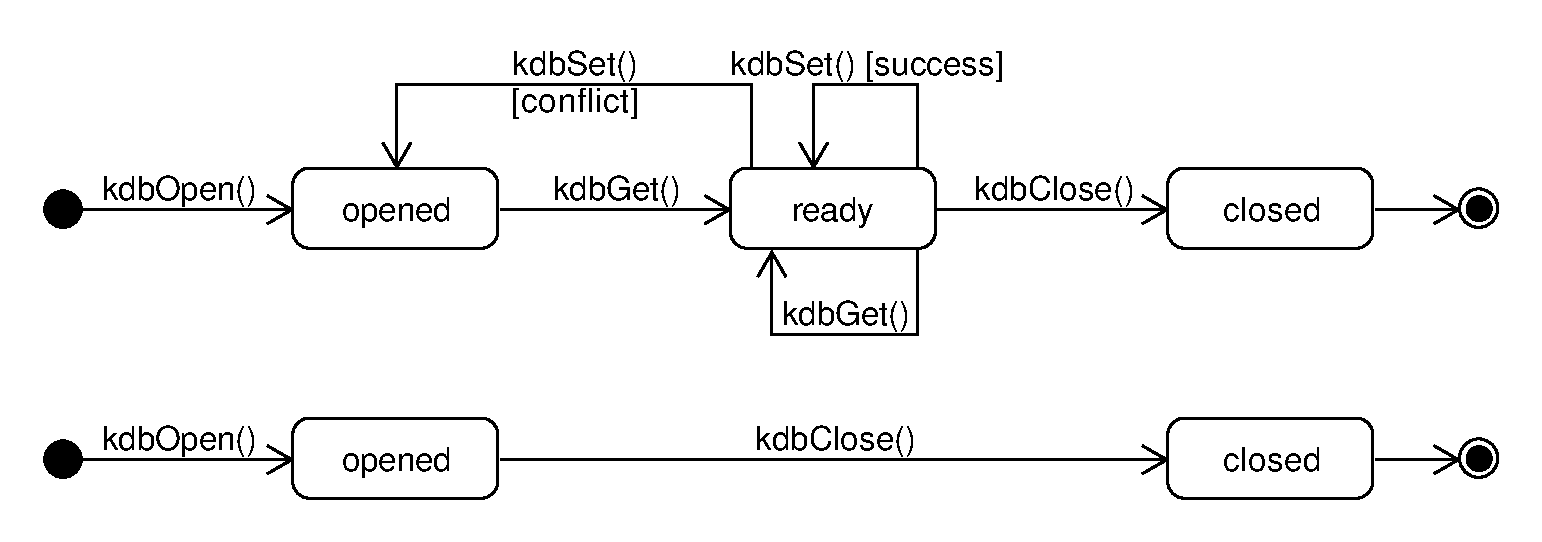
\includegraphics[width=15.0cm]{umlet-figures/impl_elektra_state.pdf}
\end{figure}

\subsection{Backend}

Backends are one or more plugins combined into a unit that interact with a single configuration file.
The backend is mounted into Elektra's configuration hierachy.
This process is similar to the mounting process in UNIX-like file systems, where a device can be mounted to a specific directory in the virtual file system.
In terms of Elektra the virtual file system is the key-value database and the device is the configuration file.
Every backend has its own configuration itself (i.e. backend configuration), which specifies the runtime behavior of the plugins within the backend.

\subsection{Compilation Variants}

Elektra's build scripts provide a functionality called \emph{compilation variants}, which means a plugin is being compiled multiple times with minor differences.
Let us demonstrate this idea using the \crypto ~as an example.
Cryptographic functions are provided by different libraries (see Section \ref{intro-provider} on page \pageref{intro-provider}) interchangeably.
The basic structure of the plugin stays the same for every compilation variant except for the library-specific calls.
These calls are encapsulated using C preprocessor directives, which form the actual compilation variants.
Listing \ref{impl-cryptoInit} on page \pageref{impl-cryptoInit} further illustrates the use of compilation variants, showing how the crypto libraries are initialized by the \crypto.

\begin{lstlisting}[label=impl-cryptoInit,language=C,caption={Example of how to use compilation variants in Elektra}]
static int elektraCryptoInit (Key * errorKey)
{
#if defined(ELEKTRA_CRYPTO_API_GCRYPT)
	return elektraCryptoGcryInit (errorKey);
#elif defined(ELEKTRA_CRYPTO_API_OPENSSL)
	return elektraCryptoOpenSSLInit (errorKey);
#elif defined(ELEKTRA_CRYPTO_API_BOTAN)
	return elektraCryptoBotanInit (errorKey);
#else
	return 1;
#endif
}
\end{lstlisting}

As we can see every crypto library is handled differently but the code frame of the plugin stays the same for all compilation variants.

\section{Crypto Plugin}\label{crypto-plugin}

\subsection{Reasons For Developing The Plugin}

In order to evaluate our research questions we need a reference application with a high degree of modularity.
The modularity is required to gain profound insight in the runtime behavior of the reference application.
By combining different Elektra plugins we can test a variety of possible use cases.

Elektra originally did not provide any cryptographic functions when we started working on this thesis.
So we choose to develop the \crypto ~for Elektra.
The \crypto ~enables us to use Elektra as benchmark environment.

\subsection{Benefits For The Elektra Project}

Elektra is a configuration database and as such it will be used for storing sensitive configuration values (for example: login credentials) at some point.
Leaving these values unencrypted is a security threat.
The \crypto{} is a way of tackling this threat by providing transparent encryption and decryption.
This means that the configuration values are stored encrypted on the filesystem and are decrypted by Elektra whenever the application requests its configuration.
Thus the encryption and the decryption work transparent to both the user and the application.
The \crypto{} can simply be added to a backend and thus integrates well with other Elektra plugins.

\subsection{Challenges}

The first challenge was to design the \crypto ~in a way that supports more than one provider of cryptographic functions.
With the goal of comparability in mind, the encryption and decryption schema will be similar for each provider.
Otherwise no conclusions can be drawn from differing benchmark results.
Elektra's compilation variants enable the support for multiple providers.
For every provider we want to integrate, a new compilation variant is added to the \crypto.

The next problem was how to generate, derive and restore the keys for the cryptographic functions.
This part of the plugin is crucial from a security perspective.
Any kind of wrongdoing in this module could lead to leaks, endangering the confidentiality of the protected data.
The first design that came to mind was a password based schema that utilizes the Password-Based Key Derivation Function 2 (PBKDF2).\footnote{PBKDF2 is specified in RFC 2898.}
However, this approach is not suitable for any kind of batch operation as the program flow would be interrupted to ask for a password input.
So we decided to delegate the handling of cryptographic keys to an existing key store: GnuPG.
GnuPG in combination with the \texttt{pinentry} utilities turned out to be a great way of managing keys.
In addition the users benefit from this approach because they can simply use their existing PGP keys and even smart-cards for securing their data in Elektra.

In the following section we are going to dive deeper into the technical details of the implementation of the \crypto.

\subsection{Technical Aspects}

The \crypto{} acts as a filter that is applied to the configuration setting before the storage plugin reaches its \texttt{kdb set} phase.
Later on, when the encrypted configuration is requested, the plugin decrypts the configuration setting after the storage plugin read the configuration file in its \texttt{kdb get} phase.
Figure \ref{impl_crypto_overview} on page \pageref{impl_crypto_overview} further illustrates how the process works.

\begin{figure}[h]
\center
\caption{Crypto Plugin: Overview of the encryption and decryption process}
\label{impl_crypto_overview}
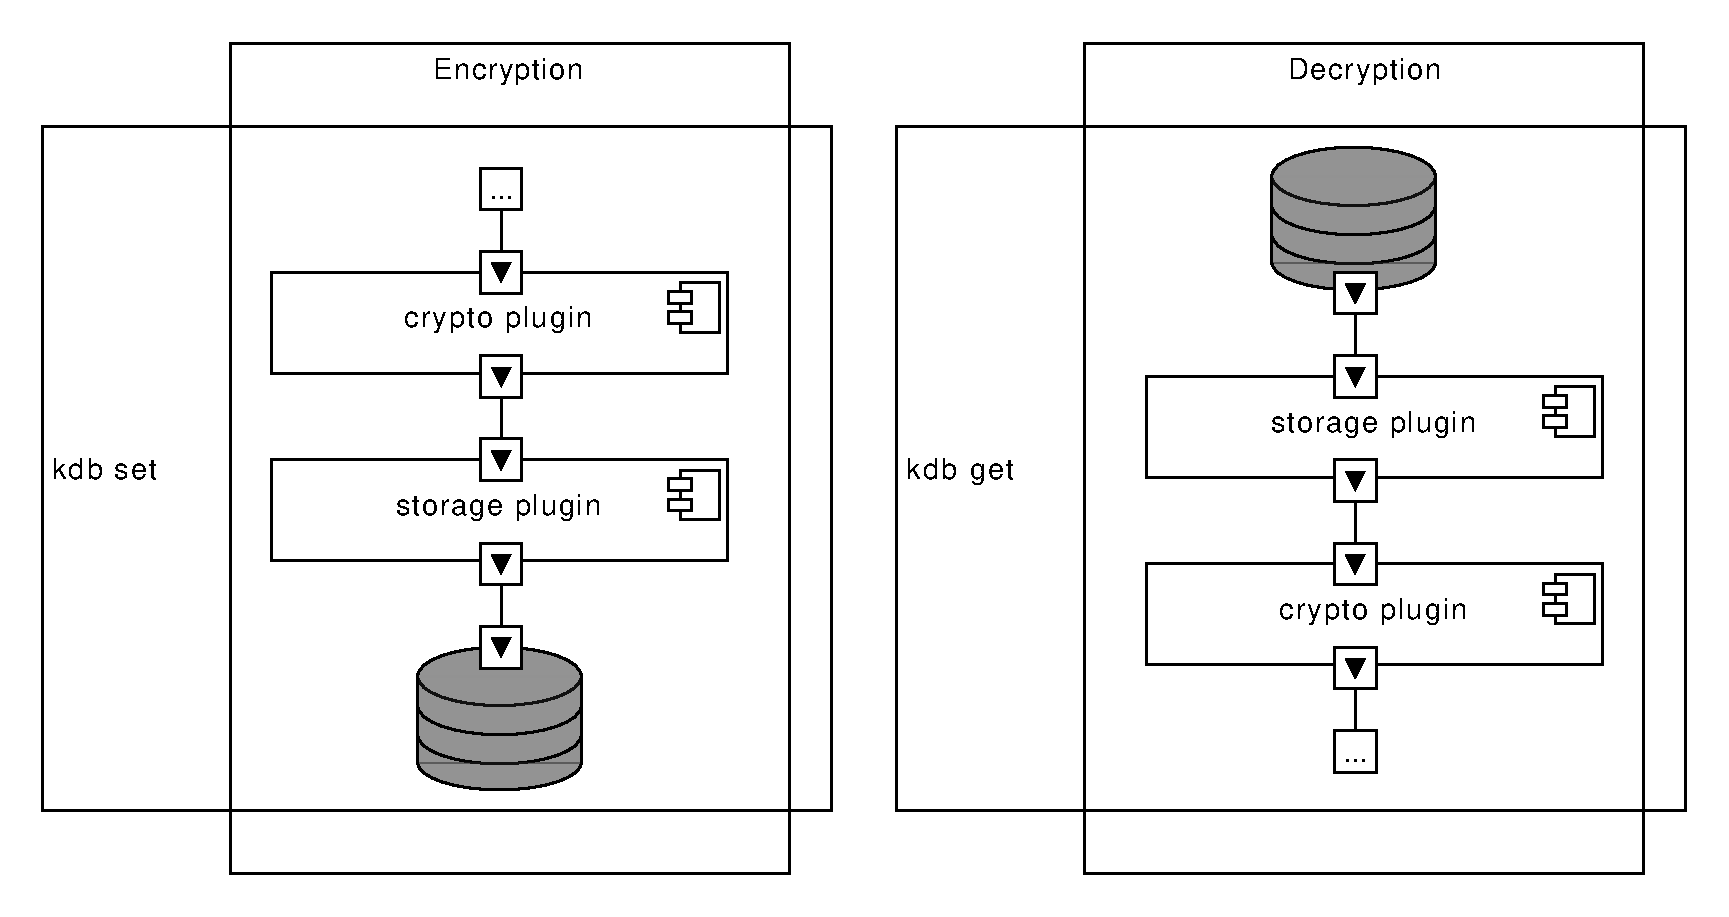
\includegraphics[width=15.0cm]{umlet-figures/impl_crypto_overview.pdf}
\end{figure}

Not all configuration values in the configuration setting are considered for encryption or decryption.
The \crypto{} uses a metakey to identify which configuration values have to be processed.
If a metakey with name \texttt{``crypto/encrypt''} is set to a value of \texttt{``1''} then the configuration value is marked for encryption.
The plugin checks the metakey and only encrypts values if the metakey is set properly.
The decryption works analogous.
All other configuration values, which are not marked, are ignored and left unchanged by the \crypto.

\subsection{Cryptographic Details}

In this section we elaborate the details of how the encryption and decryption process works.

\subsubsection{Data Structures}

The \crypto ~defines a single data structure, which is propagated throughout the plugin:

\paragraph{elektraCryptoHandle} is a structure that abstracts the library specific data types which hold keys and initialization data for the cryptographic functions.

Listing \ref{list-elektraCryptoHandle} on page \pageref{list-elektraCryptoHandle} shows the definition of the \texttt{elektraCryptoHandle} for the OpenSSL plugin variant.

\begin{lstlisting}[label=list-elektraCryptoHandle,language=C,caption={Definiton of elektraCryptoHandle for the OpenSSL crypto plugin variant}]
typedef struct
{
	EVP_CIPHER_CTX * encrypt;
	EVP_CIPHER_CTX * decrypt;
} elektraCryptoHandle;
\end{lstlisting}


\subsubsection{Message Structure}
\label{impl-msgstruct}

The \crypto{} operates on configuration values.
During its work it modifies the value as well as the meta-data.
The value is always transformed into binary data.
In order to restore the value to its original type during decryption, some header information has to be stored.

Table \ref{impl-msgheader} on page \pageref{impl-msgheader} shows the information which is encoded into the first cryptographic block during encryption.

\begin{table}[h]
\centering
\caption{Structure of the crypto message header}
\label{impl-msgheader}
\begin{tabular}{lrrlc}
	\textbf{element}           & \textbf{offset} & \textbf{length} & \textbf{data type}    & \textbf{encrypted} \\ \hline
	magic number ``\#!crypto'' & 0               & 8 B             & character             & no                 \\
	payload version            & 8               & 2 B             & character             & no                 \\
	length of the salt $L_S$   & 10              & 4 B             & unsigned long integer & no                 \\
	salt                       & 14              & $L_S$ B         & byte                  & no                 \\
	original data type         & 14 + $L_S$      & 1 B             & byte                  & yes                \\
	original content length    & 15 + $L_S$      & 4 B             & unsigned long integer & yes                \\ \hline
\end{tabular}
\end{table}

The salt is a sequence of random bytes and is used in cryptography to prevent table-based key guessing attacks.
The content length is saved because most provider of cryptographic functions do not support padding out of the box, which means that they always operate on whole blocks of data, where the block size depends on the cryptographic algorithm that is used.

\subsubsection{Key Derivation}

As mentioned before, GnuPG is used for managing the users' asymmetric keys.
GnuPG is executed to store and receive a \emph{master password}, which is a part of the plugin configuration of the \crypto.
Whenever a cryptographic key is required, the master password is fetched from the plugin configuration and decrypted.
Then the PBKDF2 is applied to the decrypted master password together with a salt, so that a cryptographic key as well as an initialization vector can be derived.

\subsubsection{Crypto Plugin Methods}

The \crypto ~implements Elektra's plugin methods (see Section \ref{impl-method-checkconf} on page \pageref{impl-method-checkconf}).
In the following section the program flow of the plugin methods is explained.

\paragraph*{open}
initializes the provider of cryptographic functions.

\paragraph*{close}
properly shuts down the provider of cryptographic functions.

\paragraph*{get}
The \texttt{get} method takes a configuration setting as input.
The \crypto ~iterates over the configuration setting and checks for every configuration value if it has been encrypted.
This is done by using the metakey mentioned before.
If the configuration value is encrypted, the \crypto ~decrypts it and thus restores the configuration value to the state it was in before the encryption took place.

Figure \ref{impl_decrypt} on page \pageref{impl_decrypt} illustrates how the \texttt{get} method works in detail.

\begin{figure}[h]
\center
\caption{Crypto Plugin: Decryption of a keyset at the kdb get method}
\label{impl_decrypt}
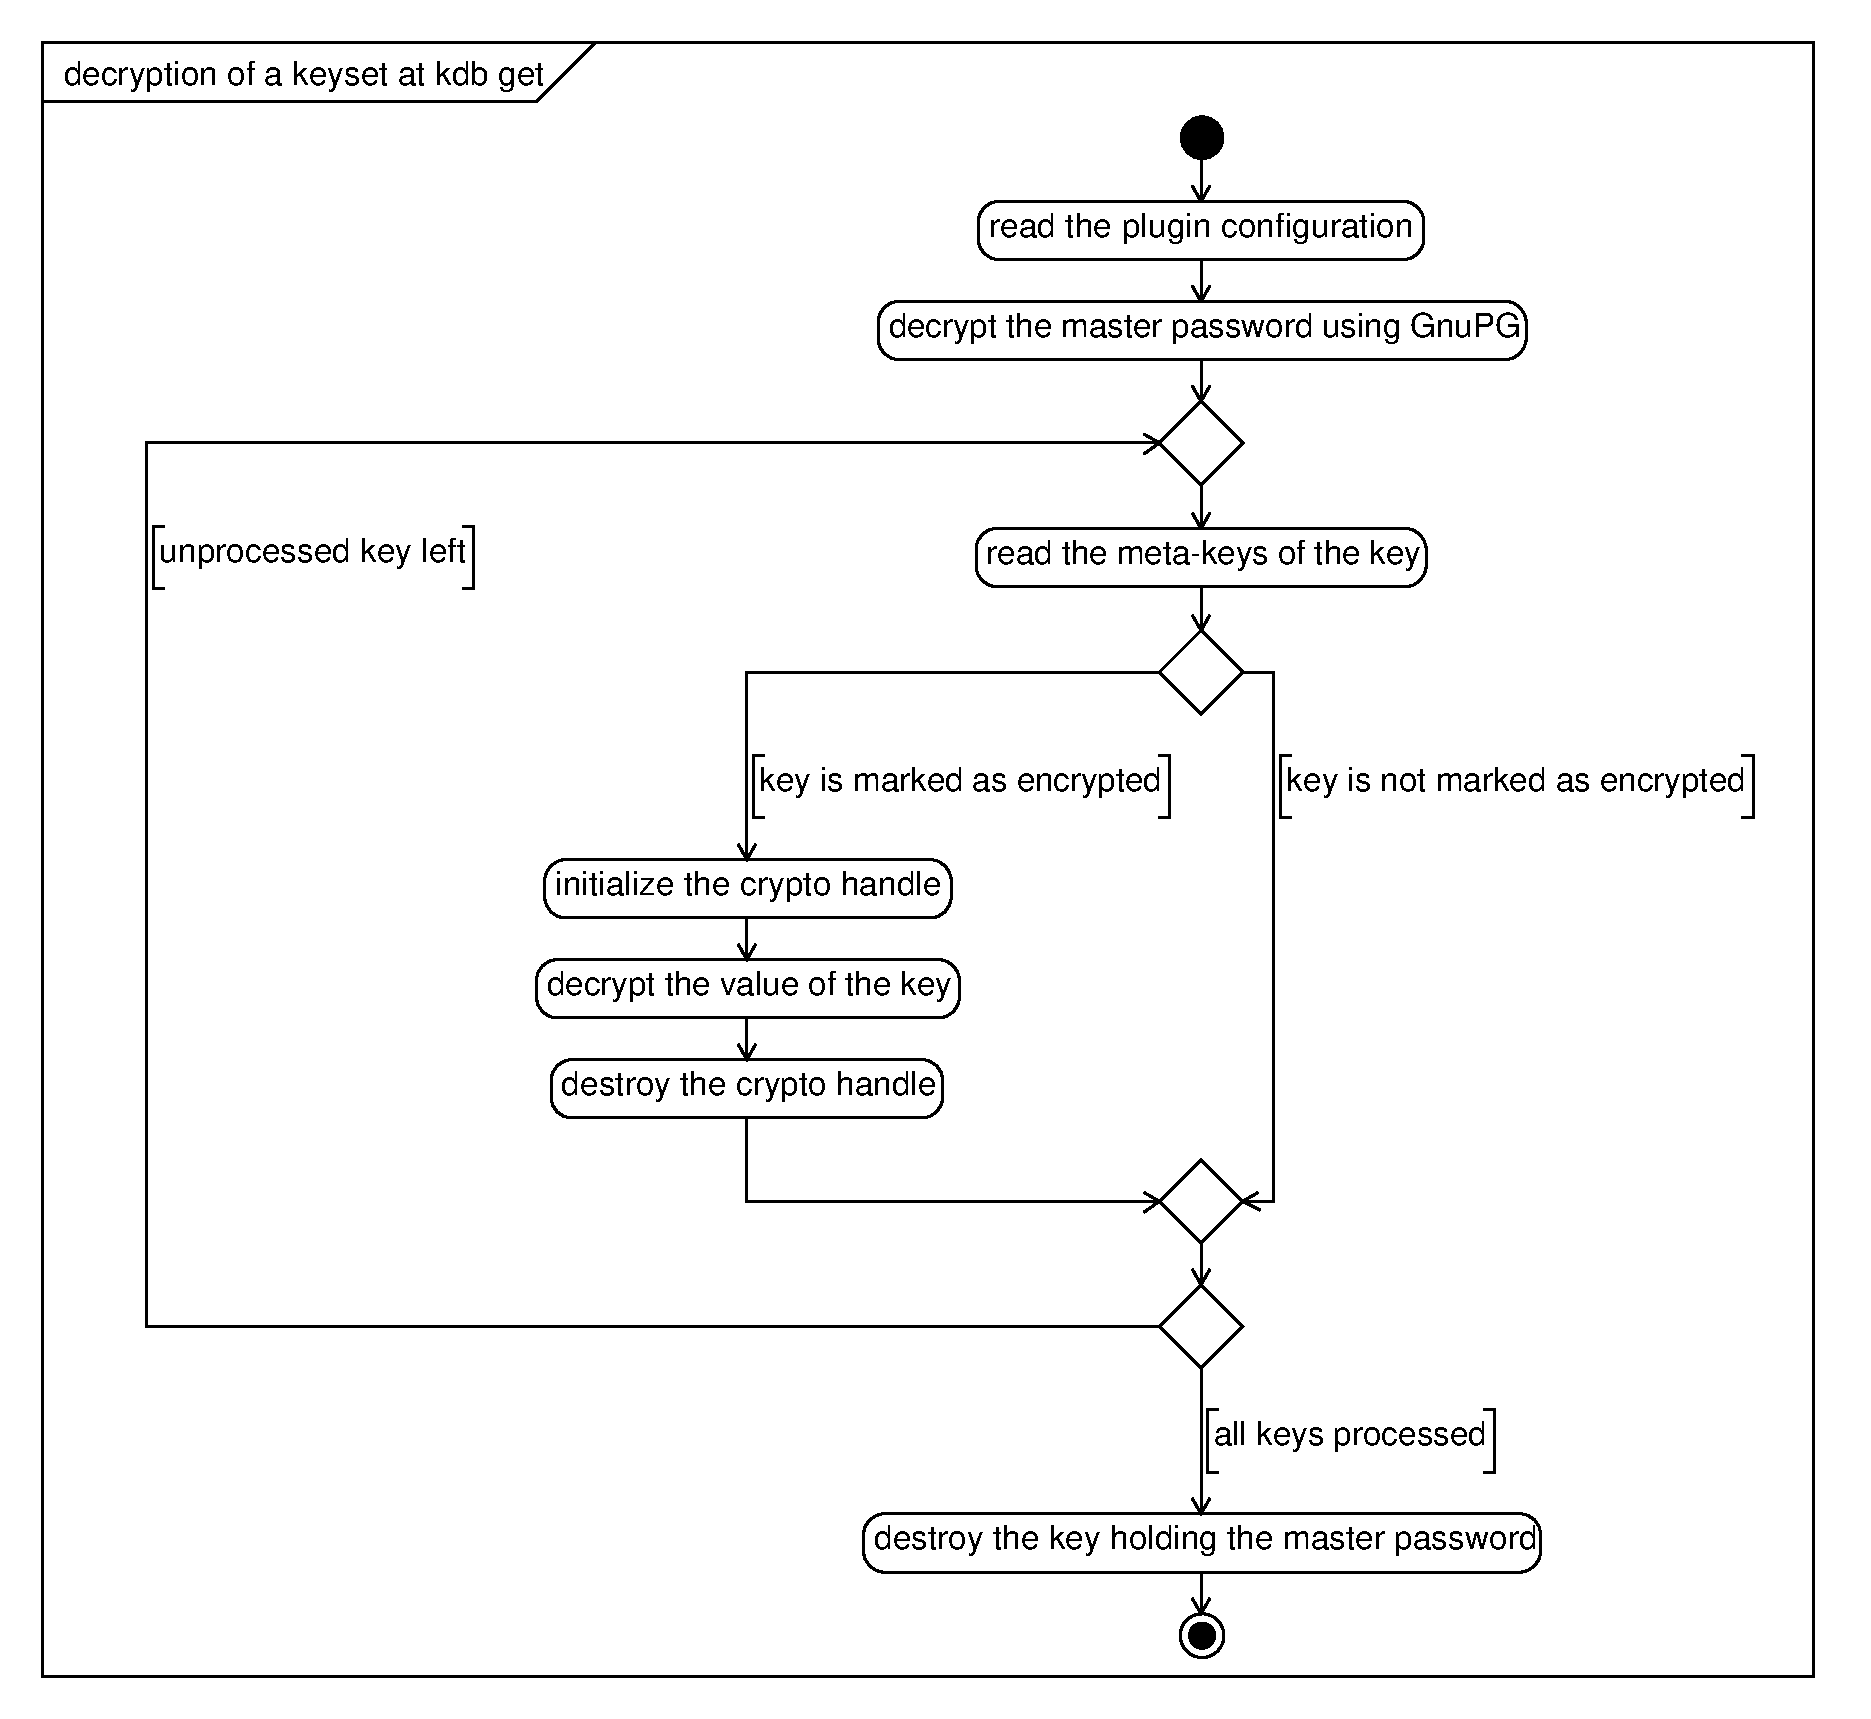
\includegraphics[width=15.0cm]{umlet-figures/impl_decrypt.pdf}
\end{figure}


\paragraph*{set}
The \texttt{set} method takes a configuration setting as input.
The \crypto ~iterates over the configuration setting and checks every configuration value if it has been marked for encryption.
Marking a configuration value for encryption is done by using a metakey.
If the metakey is present, the \crypto ~generates a message header (see Section \ref{impl-msgstruct} on page \pageref{impl-msgstruct}) including a random salt and encrypts the configuration value.

Figure \ref{impl_encrypt} on page \pageref{impl_encrypt} illustrates how the \texttt{set} method works in detail.

\begin{figure}[h]
\center
\caption{Crypto Plugin: Encryption of a keyset at the kdb set method}
\label{impl_encrypt}
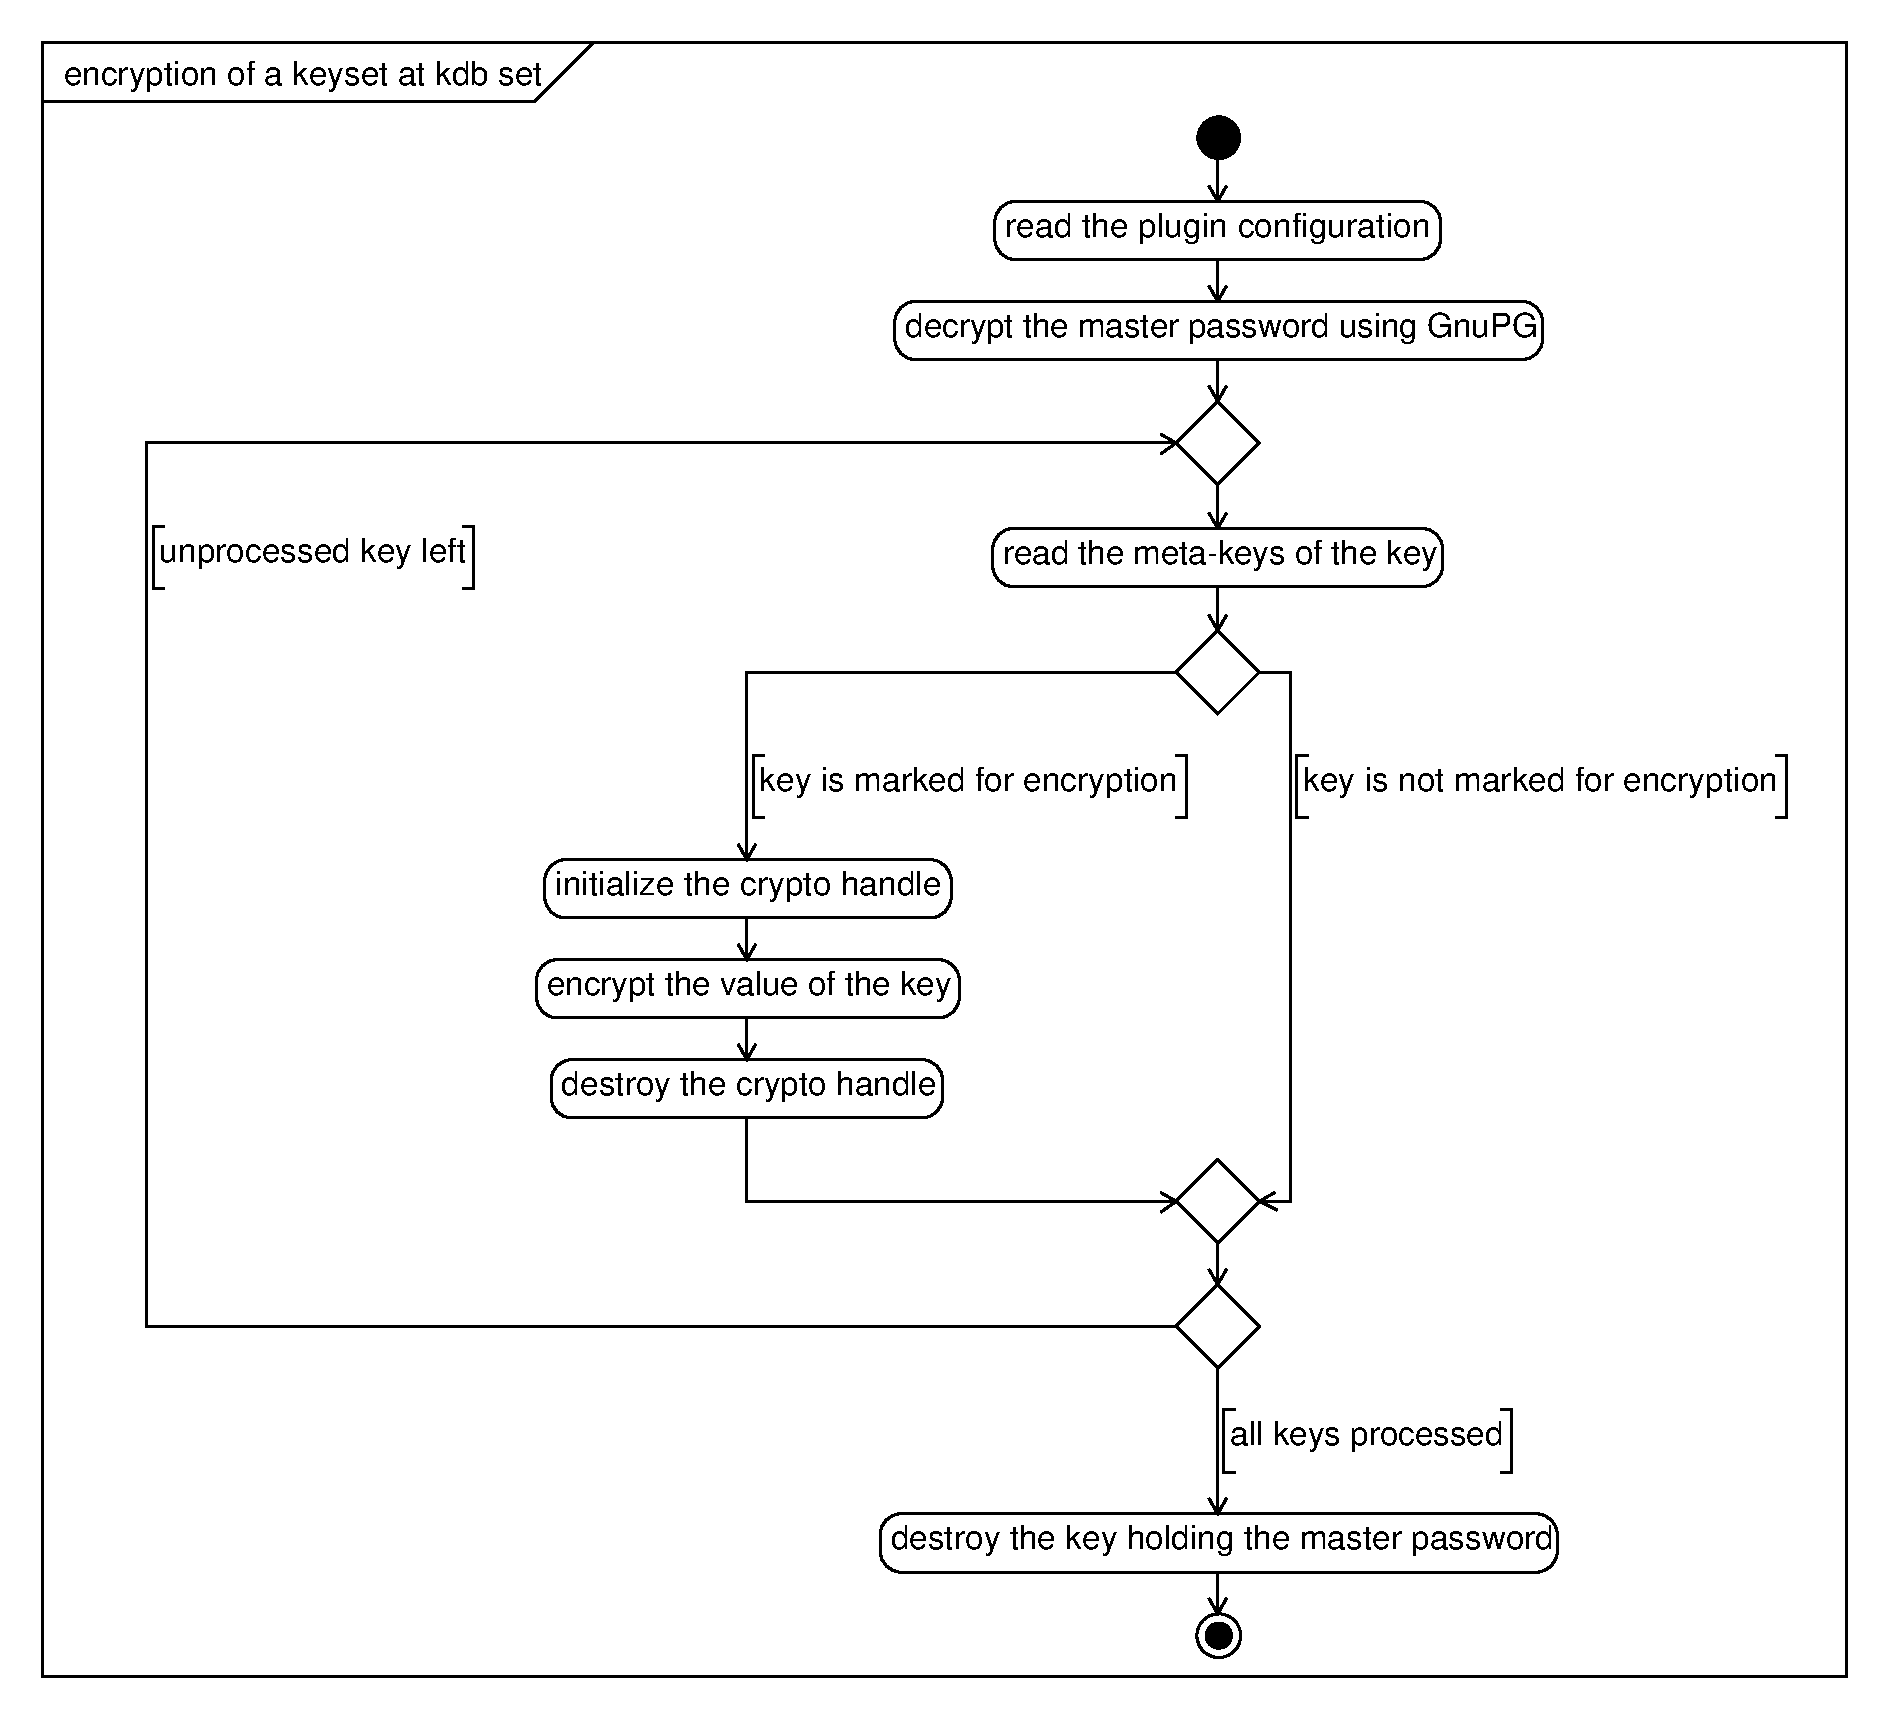
\includegraphics[width=15.0cm]{umlet-figures/impl_encrypt.pdf}
\end{figure}

\paragraph*{checkconf}
The \texttt{checkconf} method ensures that a master password is available in the plugin configuration of the \crypto.
If an encrypted master password is provided, a decryption run is started to see if the user owns the required GnuPG key.
Otherwise, a random master password is created, encrypted using GnuPG and stored in the plugin configuration.
The encryption key has to be specified within the plugin configuration.
If no such GnuPG private key is specified, the \crypto ~throws an error.

Figure \ref{impl_checkconf} on page \pageref{impl_checkconf} illustrates how the \texttt{checkconf} method works in detail.

\begin{figure}[h]
\center
\caption{Crypto Plugin: the kdb checkconf method}
\label{impl_checkconf}
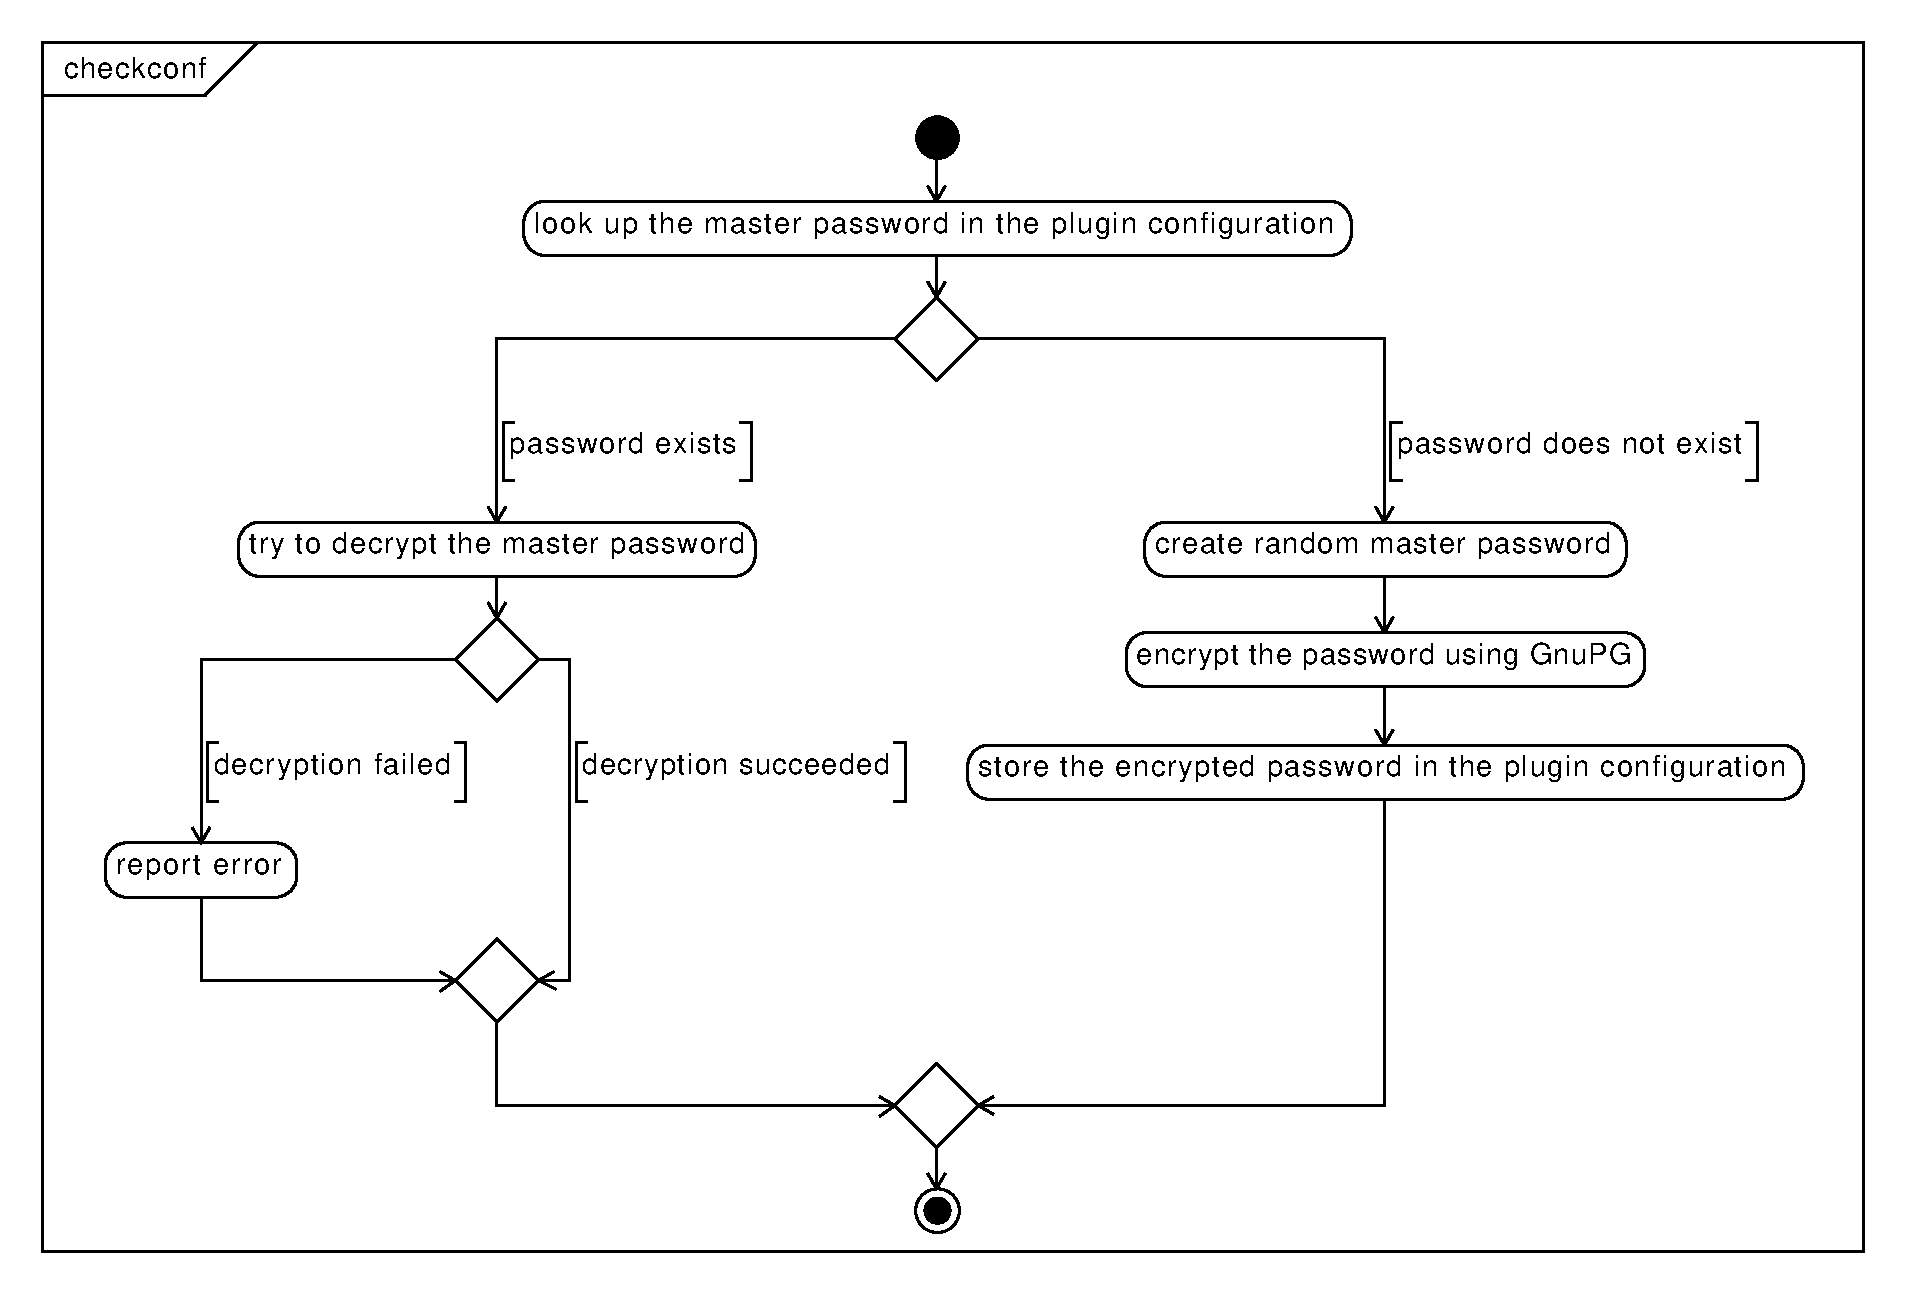
\includegraphics[width=15.0cm]{umlet-figures/impl_checkconf.pdf}
\end{figure}

\subsubsection{Compilation Variants}

For every provider of cryptographic functions (see Section \ref{intro-provider} on page \pageref{intro-provider}) a compilation variant of the \crypto ~is created.
The following compilation variants exist:
\begin{enumerate}
	\item \texttt{crypto\_botan} for the Botan library
	\item \texttt{crypto\_gcrypt} for libgcrypt
	\item \texttt{crypto\_openssl} for the OpenSSL library
\end{enumerate}

\subsection{Details About The Crypto Libraries}\label{details-about-the-crypto-libraries}



\section{Fcrypt Plugin}\label{fcrypt-plugin}

\subsection{Reasons For Developing The Plugin}

% crypto not good for entire config files -> too much overhead
% other performance benchmark -> GPG also uses libgcrypt

\subsection{Benefits for the Elektra Project}

% Users can encrypt entire configuration files
% no compile-time dependency which is nice for developers

\subsection{Challenges}

% Elektras internal API -> sync plugin workaround

\subsection{Technical Aspects}

% cryptographic operations are entirely handled by GnuPG


The \fcrypt{} was written to encrypt and decrypt whole files using the GPG interface mentioned before.
One of its advantages is that there are no dependencies at compile time.
Only the \texttt{gpg2} or \texttt{gpg} binaries are required as runtime dependency.

Again the GPG keys to be used for encryption are defined in the plugin configuration following the same semantics as the \crypto{}.


\section{Base64 Plugin}\label{base64-plugin}

% Chapter Outro

This chapter explained the Elektra plugin system and how we used it to introduce cryptographic methods to the Elektra project.
Now that we have an application to examine, we continue with the description of the actual measurements in the following chapter.

\chapter{Experimental Evaluation}

%\section{Methodology}

The focus of this chapter is:
\begin{enumerate}
\item how the benchmark system is set up
\item the exact definition and explanation how the benchmarks work and what is measured
\item the results of the benchmarks
\end{enumerate}

%The runtime of a benchmark will be measured using the system time, which is returned by the \texttt{gettimeofday ()} system function.
%
%The memory usage is examined using the ``Massif'' tool which is part of the \texttt{valgrind} suite.\cite{valgrind}

\section{Benchmark System Setup}
  \subsection{Hardware Setup}

The processor of the benchmark system is an Intel\textregistered~ Core\texttrademark~ i7-4771 CPU clocked at 3.50 GHz with 4 cores and hyperthreading enabled (which means 8 threads are available).
The benchmark system has a total of 16 GB of DDR3 RAM clocked at 1333 MHz available.

The root partition of the operation system is located on a ``Samsung SSD 840'' solid state drive (SSD).
It is installed on a ZFS filesystem.

The \texttt{diskinfo} program gives an idea of how much throughput the SSD can handle:

\begin{lstlisting}[caption={Disk performance on the benchmark system}]
Seek times:
  Full stroke:      250 iter in   0.014774 sec =    0.059 msec
  Half stroke:      250 iter in   0.012662 sec =    0.051 msec
  Quarter stroke:   500 iter in   0.024154 sec =    0.048 msec
  Short forward:    400 iter in   0.018797 sec =    0.047 msec
  Short backward:   400 iter in   0.018726 sec =    0.047 msec
  Seq outer:       2048 iter in   0.075078 sec =    0.037 msec
  Seq inner:       2048 iter in   0.074593 sec =    0.036 msec

Transfer rates:
  outside:       102400 kbytes in   0.221568 sec =   462161 kbytes/sec
  middle:        102400 kbytes in   0.218275 sec =   469133 kbytes/sec
  inside:        102400 kbytes in   0.217949 sec =   469835 kbytes/sec
\end{lstlisting}

All benchmarks are performend on the SSD.

  \subsection{Software Setup}

The operating system FreeBSD version 11.1 with patch level 1 is used to run the benchmarks.
Elektra \todo{version} at the git commit \todo{commit-nr} is installed inside a FreeBSD jail.\footnote{FreeBSD jails
are documented at \url{https://www.freebsd.org/doc/en_US.ISO8859-1/books/handbook/jails.html}.
}
The exact setup of the benchmark jail is explained in appendix \ref{jail-setup} on page \pageref{jail-setup}.

The most important program versions are listed below:

\begin{itemize}
  \item FreeBSD clang version 4.0.0 (tags/RELEASE\_400/final 297347) (based on LLVM 4.0.0)
  \item Botan version 1.10.13\_3
  \item OpenSSL version 1.0.2k-freebsd
  \item libgcrypt version 1.8.0
  \item GnuPG version 2.1.21
\end{itemize}

In the following section the benchmarks are documented and explained in detail.

\section{Benchmark 1 -- TBD}

\section{Interpretation Of The Results}

\chapter{Related and Future Work}

\section{Related Work}\label{relatedwork}

Performance analysis of cryptographic operations has already been studied in different contexts.

	\subsection{Comparing AES Implementations}

The paper ''DES, AES and Blowfish: Symmetric Key Cryptography Algorithms Simulation Based Performance Analysis`` \cite{thakur2011aes} compares implementations of symmetric cryptographic algorithms.
The authors' goal is to find the most performant algorithm.
However, the paper does not answer how much overhead the introduction of cryptographic methods actually costs.\cite{thakur2011aes}

	\subsection{Cryptography in Operating Systems}

In ''The Design of the OpenBSD Cryptographic Framework`` \cite{ocf} developers of OpenBSD describe their kernel interface that abstracts the use of hardware accelerated cryptographic operations.
The authors mainly argue about the performance gain the OCF brings to applications.
But rather than concentrating on a single application the focus of the paper is overall system performance in scenarios where multiple applications perform cryptographic operations simultaneously.
Another aspect the paper covers is the load-balancing capability OCF has to offer, if multiple hardware acceleration cards are available on a system.

The paper's focus is the kernel and operating system performance rather than single application performance.
The paper measures speed-up in comparison to cryptographic operations performed in user-space.\cite{ocf}

''Improving High-Bandwidth TLS in the FreeBSD kernel`` \cite{freebsdtls}, another performance study, has been conducted by FreeBSD developers.
They tried to get higher TLS throughput on their high-performance network appliances for Netflix, a video on-demand streaming service.
The focus of the paper is the networking aspect considering different network adapters and tuning options in the FreeBSD kernel.
Again the focus is not a single application but rather the improvement of the TLS stack in the FreeBSD operating system.\cite{freebsdtls}

%	\subsection{Cryptography in Configuration}
%
%Because none of the mentioned papers answered our research questions, it is reasonable to perform an experimental evaluation.

\section{Future Work}

In this section we suggest further research topics, which we could not cover within this thesis.

	\subsection{Cryptographic Schemas without GnuPG}

GnuPG is a great solution for cryptographic systems, because of its key handling capabilities and its integration with Smart Cards.
However, other cryptographic schmeas should be inspected and evaluated as well.

An example of another key handling form is to use simple key files.
This method may be less secure but may be much faster than the GnuPG based cryptographic schema.

	\subsection{Other criteria for choosing providers of cryptographic functions}

Performance is not the only factor to be taken into account when choosing a provider of cryptographic functions.
Robustness against attacks (for example: side channel attacks) and correctness of the code are two important dimensions, that should also be considered.

Also the usability and the user acceptance play an important role in the decision process.
We did not cover any of those aspects due to the limited context of the thesis.

	\subsection{Signature}

\todo{Cover signatures}

\chapter{Conclusions}

\section{Résumé}

\section{Further Work}



\appendix
%\chapter{Setting up the Benchmark Jail in FreeBSD 11}
\label{jail-setup}

This chapter covers the installation of the benchmark environment in FreeBSD 11.1 using the \texttt{tcsh} shell.

\section*{Preparation of the Host System}

The jail is put on a separate ZFS dataset.

\begin{lstlisting}[language=bash]
zfs create -o mountpoint=/usr/jail ROOT/jail
setenv DESTDIR /usr/jail
\end{lstlisting}

The jail requires a network alias on the host system, otherwise netowrking will not be available within the jail.
Also a DNS server must be provided to enable package installation.

\begin{lstlisting}[language=bash]
setenv JAIL_IP 10.0.2.16
ifconfig em0 $JAIL_IP netmask 255.255.255.0 alias
echo "nameserver 192.168.0.1" >> $DESTDIR/etc/resolv.conf
\end{lstlisting}

The FreeBSD installation media has to be mounted. Then the base system can be extracted into the root directory of the jail.

\begin{lstlisting}[language=bash]
setenv BSDISO /dev/`mdconfig -f ~/FreeBSD-11.1-RELEASE-amd64-disc1.iso`
mount -t cd9660 $BSDISO /mnt
tar -xf /mnt/usr/freebsd-dist/base.txz -C $DESTDIR
tar -xf /mnt/usr/freebsd-dist/src.txz -C $DESTDIR
\end{lstlisting}

After the system is extracted, we update it to the latest patch level.

\begin{lstlisting}[language=bash]
freebsd-update -b $DESTDIR fetch
freebsd-update -b $DESTDIR install
\end{lstlisting}

Another requirement for the jail is the availability of the \texttt{devfs} filesystem.

\begin{lstlisting}[language=bash]
mount -t devfs devfs $DESTDIR/dev
\end{lstlisting}

\section*{Configuration of the Jail}

The jail is now ready to start.

\begin{lstlisting}[language=bash]
jail $DESTDIR elektra $JAIL_IP tcsh
\end{lstlisting}

The first step in the jail is the package installation.

\begin{lstlisting}[language=bash]
pkg install gnupg \
llvm40 \
botan110 \
openssl \
cmake \
git \
pkgconf \
ninja
\end{lstlisting}

Then the build process of \texttt{libelektra} can start.

\begin{lstlisting}[language=bash]
git clone https://github.com/ElektraInitiative/libelektra.git /libelektra

cd /libelektra
mkdir build && cd build

cmake \
  -GNinja \
  -DBUILD_STATIC=OFF \
  -DPLUGINS="ALL" \
  -DBINDINGS=ALL \
  -DTOOLS=ALL \
  ..

ninja
ninja install
\end{lstlisting}

The jail is now configured and ready to execute the benchmarks.

\section*{Final Step}

After the benchmark has executed, the jail environment has to be restored to its original state.
In order to be able to restore the jail, a ZFS snapshot is created.

\begin{lstlisting}[language=bash]
zfs snapshot ROOT/jail@original
\end{lstlisting}

% NOTE this file has been generated
% I would suggest to not change it manually
\chapter{Benchmark 1 Results}
\begin{sidewaystable} \centering \caption{No crypto plugin / kdb get benchmark results} \label{eval-table-no-crypto-get} \scriptsize \begin{tabular}{r|rrrrrrrrrrr} size ($n$) & run 1 & run 2 & run 3 & run 4 & run 5 & run 6 & run 7 & run 8 & run 9 & run 10 & run 11\\ \hline
$1$ & $0.000108$ & $0.000109$ & $0.000112$ & $0.000109$ & $0.000104$ & $0.000116$ & $0.000108$ & $0.000106$ & $0.000108$ & $0.000107$ & $0.000107$ \\
$2$ & $0.000109$ & $0.000111$ & $0.000118$ & $0.000113$ & $0.000129$ & $0.000114$ & $0.000112$ & $0.000112$ & $0.000141$ & $0.000112$ & $0.000112$ \\
$3$ & $0.000113$ & $0.000113$ & $0.000141$ & $0.000131$ & $0.000118$ & $0.000113$ & $0.000111$ & $0.000129$ & $0.000110$ & $0.000110$ & $0.000111$ \\
$4$ & $0.000121$ & $0.000117$ & $0.000114$ & $0.000142$ & $0.000118$ & $0.000121$ & $0.000116$ & $0.000118$ & $0.000144$ & $0.000118$ & $0.000114$ \\
$5$ & $0.000125$ & $0.000120$ & $0.000120$ & $0.000122$ & $0.000120$ & $0.000117$ & $0.000117$ & $0.000116$ & $0.000118$ & $0.000120$ & $0.000124$ \\
$6$ & $0.000123$ & $0.000124$ & $0.000128$ & $0.000125$ & $0.000121$ & $0.000126$ & $0.000124$ & $0.000127$ & $0.000121$ & $0.000124$ & $0.000127$ \\
$7$ & $0.000126$ & $0.000129$ & $0.000134$ & $0.000122$ & $0.000125$ & $0.000128$ & $0.000125$ & $0.000127$ & $0.000136$ & $0.000126$ & $0.000151$ \\
$8$ & $0.000126$ & $0.000127$ & $0.000127$ & $0.000138$ & $0.000135$ & $0.000126$ & $0.000126$ & $0.000125$ & $0.000126$ & $0.000129$ & $0.000126$ \\
$9$ & $0.000133$ & $0.000130$ & $0.000131$ & $0.000134$ & $0.000137$ & $0.000130$ & $0.000135$ & $0.000135$ & $0.000162$ & $0.000135$ & $0.000141$ \\
$10$ & $0.000135$ & $0.000166$ & $0.000138$ & $0.000135$ & $0.000136$ & $0.000133$ & $0.000136$ & $0.000134$ & $0.000133$ & $0.000133$ & $0.000135$ \\
$11$ & $0.000137$ & $0.000138$ & $0.000144$ & $0.000138$ & $0.000140$ & $0.000135$ & $0.000146$ & $0.000138$ & $0.000162$ & $0.000136$ & $0.000144$ \\
$15$ & $0.000152$ & $0.000175$ & $0.000150$ & $0.000186$ & $0.000149$ & $0.000151$ & $0.000157$ & $0.000156$ & $0.000171$ & $0.000150$ & $0.000147$ \\
$17$ & $0.000156$ & $0.000155$ & $0.000160$ & $0.000188$ & $0.000155$ & $0.000158$ & $0.000189$ & $0.000155$ & $0.000159$ & $0.000157$ & $0.000154$ \\
$20$ & $0.000164$ & $0.000170$ & $0.000165$ & $0.000178$ & $0.000173$ & $0.000168$ & $0.000167$ & $0.000207$ & $0.000210$ & $0.000164$ & $0.000163$ \\
$25$ & $0.000176$ & $0.000187$ & $0.000179$ & $0.000175$ & $0.000176$ & $0.000179$ & $0.000179$ & $0.000252$ & $0.000178$ & $0.000176$ & $0.000181$ \\
$30$ & $0.000200$ & $0.000194$ & $0.000196$ & $0.000196$ & $0.000197$ & $0.000195$ & $0.000194$ & $0.000200$ & $0.000200$ & $0.000198$ & $0.000205$ \\
$31$ & $0.000313$ & $0.000199$ & $0.000198$ & $0.000196$ & $0.000204$ & $0.000238$ & $0.000222$ & $0.000223$ & $0.000196$ & $0.000209$ & $0.000198$ \\
$32$ & $0.000203$ & $0.000222$ & $0.000204$ & $0.000234$ & $0.000219$ & $0.000204$ & $0.000199$ & $0.000204$ & $0.000210$ & $0.000227$ & $0.000200$ \\
$35$ & $0.000211$ & $0.000210$ & $0.000220$ & $0.000334$ & $0.000207$ & $0.000205$ & $0.000215$ & $0.000207$ & $0.000231$ & $0.000207$ & $0.000217$ \\
$40$ & $0.000221$ & $0.000223$ & $0.000272$ & $0.000223$ & $0.000275$ & $0.000220$ & $0.000221$ & $0.000246$ & $0.000220$ & $0.000221$ & $0.000224$ \\
$50$ & $0.000251$ & $0.000251$ & $0.000289$ & $0.000251$ & $0.000250$ & $0.000305$ & $0.000253$ & $0.000286$ & $0.000250$ & $0.000249$ & $0.000306$ \\
$51$ & $0.000254$ & $0.000251$ & $0.000324$ & $0.000254$ & $0.000312$ & $0.000253$ & $0.000261$ & $0.000258$ & $0.000263$ & $0.000262$ & $0.000258$ \\
$52$ & $0.000259$ & $0.000256$ & $0.000257$ & $0.000324$ & $0.000258$ & $0.000310$ & $0.000257$ & $0.000258$ & $0.000264$ & $0.000268$ & $0.000269$ \\
$55$ & $0.000270$ & $0.000310$ & $0.000267$ & $0.000274$ & $0.000334$ & $0.000273$ & $0.000274$ & $0.000272$ & $0.000334$ & $0.000274$ & $0.000298$ \\
$56$ & $0.000275$ & $0.000347$ & $0.000341$ & $0.000275$ & $0.000273$ & $0.000268$ & $0.000341$ & $0.000278$ & $0.000270$ & $0.000282$ & $0.000279$ \\
$57$ & $0.000280$ & $0.000294$ & $0.000276$ & $0.000273$ & $0.000321$ & $0.000292$ & $0.000271$ & $0.000315$ & $0.000356$ & $0.000282$ & $0.000276$ \\
$60$ & $0.000285$ & $0.000280$ & $0.000342$ & $0.000354$ & $0.000285$ & $0.000280$ & $0.000277$ & $0.000344$ & $0.000289$ & $0.000367$ & $0.000282$ \\
$70$ & $0.000317$ & $0.000322$ & $0.000463$ & $0.000317$ & $0.000316$ & $0.000403$ & $0.000316$ & $0.000346$ & $0.000318$ & $0.000317$ & $0.000321$ \\
$80$ & $0.000339$ & $0.000414$ & $0.000354$ & $0.000423$ & $0.000338$ & $0.000421$ & $0.000353$ & $0.000341$ & $0.000344$ & $0.000354$ & $0.000338$ \\
$90$ & $0.000376$ & $0.000469$ & $0.000371$ & $0.000370$ & $0.000367$ & $0.000378$ & $0.000367$ & $0.000368$ & $0.000382$ & $0.000402$ & $0.000367$ \\
$100$ & $0.000395$ & $0.000405$ & $0.000411$ & $0.000395$ & $0.000407$ & $0.000399$ & $0.000500$ & $0.000397$ & $0.000403$ & $0.000407$ & $0.000399$ \\
$150$ & $0.000542$ & $0.000544$ & $0.000546$ & $0.000623$ & $0.000549$ & $0.000552$ & $0.000670$ & $0.000570$ & $0.000623$ & $0.000594$ & $0.000551$ \\
$175$ & $0.000621$ & $0.000620$ & $0.000623$ & $0.000623$ & $0.000619$ & $0.000615$ & $0.000618$ & $0.000615$ & $0.000622$ & $0.000617$ & $0.000737$ \\
$200$ & $0.000695$ & $0.000697$ & $0.000686$ & $0.000687$ & $0.000685$ & $0.000700$ & $0.000702$ & $0.000698$ & $0.000701$ & $0.000842$ & $0.000723$ \\
$250$ & $0.000849$ & $0.000845$ & $0.000833$ & $0.000857$ & $0.000831$ & $0.000839$ & $0.000840$ & $0.000829$ & $0.001048$ & $0.001023$ & $0.000843$ \\
$300$ & $0.000992$ & $0.000992$ & $0.001016$ & $0.000995$ & $0.001075$ & $0.000999$ & $0.001207$ & $0.000989$ & $0.001211$ & $0.000986$ & $0.000997$ \\
$350$ & $0.001137$ & $0.001385$ & $0.001138$ & $0.001152$ & $0.001276$ & $0.001141$ & $0.001276$ & $0.001160$ & $0.001137$ & $0.001140$ & $0.001403$ \\
$400$ & $0.001325$ & $0.001299$ & $0.001296$ & $0.001332$ & $0.001302$ & $0.001294$ & $0.001316$ & $0.001297$ & $0.001589$ & $0.001344$ & $0.001297$ \\
$500$ & $0.001677$ & $0.001597$ & $0.001592$ & $0.001608$ & $0.001602$ & $0.001594$ & $0.001606$ & $0.001596$ & $0.001592$ & $0.001603$ & $0.001610$ \\
$1000$ & $0.003026$ & $0.003298$ & $0.003079$ & $0.003041$ & $0.003112$ & $0.003061$ & $0.003067$ & $0.003064$ & $0.003075$ & $0.003064$ & $0.003052$ \\
\hline
\end{tabular}
\end{sidewaystable}
 
 
\begin{sidewaystable} \centering \caption{Crypto (OpenSSL) / kdb get benchmark results} \label{eval-table-openssl-get} \scriptsize \begin{tabular}{r|rrrrrrrrrrr} size ($n$) & run 1 & run 2 & run 3 & run 4 & run 5 & run 6 & run 7 & run 8 & run 9 & run 10 & run 11\\ \hline
$1$ & $0.019106$ & $0.019493$ & $0.019318$ & $0.019548$ & $0.020126$ & $0.020168$ & $0.019702$ & $0.020091$ & $0.019825$ & $0.019274$ & $0.019326$ \\
$2$ & $0.035684$ & $0.036220$ & $0.035922$ & $0.035559$ & $0.035758$ & $0.036376$ & $0.036529$ & $0.035702$ & $0.036411$ & $0.036093$ & $0.036694$ \\
$3$ & $0.052350$ & $0.051586$ & $0.051926$ & $0.052327$ & $0.052701$ & $0.052502$ & $0.052143$ & $0.051790$ & $0.052695$ & $0.052676$ & $0.052330$ \\
$4$ & $0.068674$ & $0.068509$ & $0.068932$ & $0.074033$ & $0.069303$ & $0.069261$ & $0.069081$ & $0.069448$ & $0.068821$ & $0.069099$ & $0.069629$ \\
$5$ & $0.084847$ & $0.086081$ & $0.084704$ & $0.085630$ & $0.085687$ & $0.084705$ & $0.085089$ & $0.085229$ & $0.084912$ & $0.085134$ & $0.085397$ \\
$6$ & $0.102441$ & $0.102142$ & $0.103138$ & $0.102280$ & $0.101936$ & $0.101980$ & $0.102461$ & $0.101786$ & $0.102446$ & $0.101946$ & $0.101674$ \\
$7$ & $0.118112$ & $0.117638$ & $0.118249$ & $0.119149$ & $0.118725$ & $0.119025$ & $0.118817$ & $0.118436$ & $0.118334$ & $0.118102$ & $0.119864$ \\
$8$ & $0.133952$ & $0.133147$ & $0.140413$ & $0.134206$ & $0.134669$ & $0.134158$ & $0.134187$ & $0.134948$ & $0.134566$ & $0.134245$ & $0.134310$ \\
$9$ & $0.151133$ & $0.151394$ & $0.150463$ & $0.151489$ & $0.155961$ & $0.150897$ & $0.151547$ & $0.155186$ & $0.151417$ & $0.152115$ & $0.151871$ \\
$10$ & $0.167447$ & $0.168038$ & $0.167140$ & $0.167192$ & $0.167625$ & $0.167140$ & $0.167869$ & $0.167517$ & $0.167576$ & $0.168644$ & $0.168485$ \\
$11$ & $0.183921$ & $0.183600$ & $0.188512$ & $0.184445$ & $0.186407$ & $0.183456$ & $0.184306$ & $0.183984$ & $0.183349$ & $0.183989$ & $0.183465$ \\
$15$ & $0.249082$ & $0.249136$ & $0.260151$ & $0.249046$ & $0.248899$ & $0.248819$ & $0.249553$ & $0.249795$ & $0.249688$ & $0.249218$ & $0.252313$ \\
$17$ & $0.283523$ & $0.284885$ & $0.286503$ & $0.284658$ & $0.285224$ & $0.293421$ & $0.285208$ & $0.284853$ & $0.314798$ & $0.288659$ & $0.286127$ \\
$20$ & $0.332602$ & $0.330650$ & $0.331555$ & $0.331458$ & $0.332260$ & $0.331791$ & $0.331478$ & $0.332617$ & $0.331485$ & $0.333575$ & $0.333138$ \\
$25$ & $0.415218$ & $0.414051$ & $0.413353$ & $0.417011$ & $0.412725$ & $0.413410$ & $0.413174$ & $0.419609$ & $0.413181$ & $0.414127$ & $0.424323$ \\
$30$ & $0.494789$ & $0.494597$ & $0.494073$ & $0.495479$ & $0.495719$ & $0.502185$ & $0.494462$ & $0.495492$ & $0.493701$ & $0.495446$ & $0.495085$ \\
$31$ & $0.509923$ & $0.510319$ & $0.511091$ & $0.511315$ & $0.511611$ & $0.511653$ & $0.509250$ & $0.510807$ & $0.514879$ & $0.511194$ & $0.510733$ \\
$32$ & $0.534686$ & $0.572115$ & $0.539954$ & $0.533790$ & $0.543749$ & $0.538967$ & $0.535497$ & $0.535207$ & $0.533512$ & $0.532138$ & $0.537942$ \\
$35$ & $0.576764$ & $0.585017$ & $0.575869$ & $0.576995$ & $0.576499$ & $0.577088$ & $0.577542$ & $0.584968$ & $0.577635$ & $0.576585$ & $0.582493$ \\
$40$ & $0.662732$ & $0.662353$ & $0.675167$ & $0.665267$ & $0.661621$ & $0.662293$ & $0.662191$ & $0.660319$ & $0.667363$ & $0.662734$ & $0.663024$ \\
$50$ & $0.822010$ & $0.823423$ & $0.822045$ & $0.823645$ & $0.825094$ & $0.822421$ & $0.870433$ & $0.829308$ & $0.823946$ & $0.871561$ & $0.823214$ \\
$51$ & $0.840409$ & $0.839296$ & $0.838830$ & $0.847197$ & $0.839071$ & $0.841548$ & $0.840995$ & $0.839648$ & $0.840361$ & $0.839463$ & $0.842546$ \\
$52$ & $0.918945$ & $0.924425$ & $0.917451$ & $0.916574$ & $0.916797$ & $0.922361$ & $0.917744$ & $0.917859$ & $0.918603$ & $0.916616$ & $0.916141$ \\
$55$ & $0.903981$ & $0.916233$ & $0.904484$ & $0.905156$ & $0.908645$ & $0.906397$ & $0.906629$ & $0.905451$ & $0.931994$ & $0.918168$ & $0.903719$ \\
$56$ & $0.927478$ & $0.940305$ & $0.926616$ & $0.972815$ & $0.925468$ & $0.925368$ & $0.931157$ & $0.923885$ & $0.929628$ & $0.950770$ & $0.929009$ \\
$57$ & $0.935589$ & $0.941970$ & $0.940453$ & $0.938819$ & $0.938382$ & $0.942869$ & $0.939047$ & $0.936821$ & $0.939840$ & $0.938347$ & $0.936806$ \\
$60$ & $0.987045$ & $0.986850$ & $0.985844$ & $0.985888$ & $0.985945$ & $0.986464$ & $0.987978$ & $0.986126$ & $0.990678$ & $0.988372$ & $0.988414$ \\
$70$ & $1.151348$ & $1.151068$ & $1.151429$ & $1.151822$ & $1.162766$ & $1.150500$ & $1.152885$ & $1.150049$ & $1.151203$ & $1.151578$ & $1.156338$ \\
$80$ & $1.318126$ & $1.316492$ & $1.320604$ & $1.319162$ & $1.330473$ & $1.317369$ & $1.337937$ & $1.333779$ & $1.318621$ & $1.326121$ & $1.327114$ \\
$90$ & $1.569392$ & $1.493429$ & $1.497271$ & $1.500871$ & $1.493853$ & $1.495288$ & $1.492880$ & $1.500103$ & $1.502549$ & $1.499455$ & $1.494033$ \\
$100$ & $1.645525$ & $1.643997$ & $1.641346$ & $1.638501$ & $1.674659$ & $1.644927$ & $1.638406$ & $1.644130$ & $1.637074$ & $1.784840$ & $1.642844$ \\
$150$ & $2.472021$ & $2.459184$ & $2.470929$ & $2.464726$ & $2.455564$ & $2.516300$ & $2.608414$ & $2.576765$ & $2.462609$ & $2.488534$ & $2.462541$ \\
$175$ & $3.015162$ & $3.030083$ & $3.028133$ & $3.130669$ & $3.139086$ & $3.029557$ & $3.019923$ & $3.033275$ & $3.029643$ & $3.021501$ & $3.038056$ \\
$200$ & $3.301826$ & $3.313739$ & $3.290038$ & $3.291292$ & $3.292536$ & $3.312082$ & $3.417187$ & $3.287592$ & $3.464195$ & $3.288169$ & $3.288560$ \\
$250$ & $4.099789$ & $4.103806$ & $4.227536$ & $4.099148$ & $4.102502$ & $4.102067$ & $4.102851$ & $4.130434$ & $4.101508$ & $4.099958$ & $4.095367$ \\
$300$ & $4.915201$ & $4.926065$ & $4.928836$ & $4.930378$ & $4.928449$ & $5.038341$ & $4.921983$ & $4.976804$ & $4.919224$ & $4.919849$ & $4.921130$ \\
$350$ & $5.808056$ & $5.834985$ & $5.808688$ & $5.913375$ & $5.796697$ & $5.806803$ & $5.823371$ & $6.357305$ & $5.803105$ & $5.757831$ & $5.741849$ \\
$400$ & $6.583391$ & $6.572334$ & $6.565796$ & $6.615653$ & $6.551437$ & $6.566439$ & $6.553900$ & $6.548495$ & $6.570032$ & $6.622150$ & $6.581622$ \\
$500$ & $8.207802$ & $8.275084$ & $8.190037$ & $8.266980$ & $8.303596$ & $8.279787$ & $8.198080$ & $8.232770$ & $8.189081$ & $8.225321$ & $8.274256$ \\
$1000$ & $16.657685$ & $16.423004$ & $16.714214$ & $16.659074$ & $16.490285$ & $16.576172$ & $16.658430$ & $16.639539$ & $16.586751$ & $16.582807$ & $16.663801$ \\
\hline
\end{tabular}
\end{sidewaystable}
 
 
\begin{sidewaystable} \centering \caption{Crypto (libgcrypt) / kdb get benchmark results} \label{eval-table-libgcrypt-get} \scriptsize \begin{tabular}{r|rrrrrrrrrrr} size ($n$) & run 1 & run 2 & run 3 & run 4 & run 5 & run 6 & run 7 & run 8 & run 9 & run 10 & run 11\\ \hline
$1$ & $0.013730$ & $0.013484$ & $0.013708$ & $0.014000$ & $0.014211$ & $0.013785$ & $0.014222$ & $0.014041$ & $0.014320$ & $0.013771$ & $0.013528$ \\
$2$ & $0.024070$ & $0.024367$ & $0.024022$ & $0.023993$ & $0.024328$ & $0.024281$ & $0.024542$ & $0.024392$ & $0.024869$ & $0.025458$ & $0.024741$ \\
$3$ & $0.035580$ & $0.034636$ & $0.034597$ & $0.034477$ & $0.035350$ & $0.034588$ & $0.034504$ & $0.034943$ & $0.035474$ & $0.034947$ & $0.035927$ \\
$4$ & $0.045772$ & $0.046404$ & $0.045611$ & $0.046841$ & $0.045713$ & $0.045820$ & $0.045619$ & $0.046450$ & $0.046495$ & $0.047260$ & $0.047127$ \\
$5$ & $0.055820$ & $0.055473$ & $0.055904$ & $0.056125$ & $0.056056$ & $0.055458$ & $0.055816$ & $0.055780$ & $0.056071$ & $0.055658$ & $0.056513$ \\
$6$ & $0.066766$ & $0.067075$ & $0.066860$ & $0.067385$ & $0.067394$ & $0.067043$ & $0.067718$ & $0.066707$ & $0.067502$ & $0.066492$ & $0.067133$ \\
$7$ & $0.078110$ & $0.079494$ & $0.077851$ & $0.079546$ & $0.078842$ & $0.078304$ & $0.077610$ & $0.078357$ & $0.078030$ & $0.078233$ & $0.079471$ \\
$8$ & $0.087530$ & $0.087337$ & $0.088155$ & $0.087230$ & $0.088599$ & $0.087910$ & $0.087949$ & $0.087380$ & $0.087932$ & $0.087596$ & $0.087406$ \\
$9$ & $0.100666$ & $0.099023$ & $0.099446$ & $0.099264$ & $0.101758$ & $0.099140$ & $0.099429$ & $0.098827$ & $0.099444$ & $0.099198$ & $0.099459$ \\
$10$ & $0.110525$ & $0.111025$ & $0.109811$ & $0.111592$ & $0.110206$ & $0.111081$ & $0.109951$ & $0.111354$ & $0.111349$ & $0.110539$ & $0.110328$ \\
$11$ & $0.121379$ & $0.120430$ & $0.120388$ & $0.120077$ & $0.122913$ & $0.119988$ & $0.120487$ & $0.120630$ & $0.122750$ & $0.120623$ & $0.120545$ \\
$15$ & $0.161763$ & $0.161754$ & $0.161971$ & $0.161629$ & $0.162263$ & $0.161714$ & $0.162361$ & $0.162586$ & $0.162741$ & $0.162213$ & $0.162502$ \\
$17$ & $0.188489$ & $0.188672$ & $0.188284$ & $0.188403$ & $0.188163$ & $0.193918$ & $0.188686$ & $0.188895$ & $0.189179$ & $0.188962$ & $0.188427$ \\
$20$ & $0.216675$ & $0.217360$ & $0.217387$ & $0.219036$ & $0.217022$ & $0.217180$ & $0.218270$ & $0.217292$ & $0.217095$ & $0.219029$ & $0.218079$ \\
$25$ & $0.272339$ & $0.271415$ & $0.272376$ & $0.270480$ & $0.271116$ & $0.270834$ & $0.271080$ & $0.271225$ & $0.271863$ & $0.272501$ & $0.272616$ \\
$30$ & $0.320788$ & $0.320142$ & $0.320362$ & $0.320476$ & $0.320430$ & $0.320701$ & $0.339904$ & $0.320651$ & $0.320694$ & $0.320649$ & $0.320808$ \\
$31$ & $0.331344$ & $0.332289$ & $0.331868$ & $0.334133$ & $0.334437$ & $0.331229$ & $0.331258$ & $0.330699$ & $0.333062$ & $0.334636$ & $0.336529$ \\
$32$ & $0.344131$ & $0.344160$ & $0.344912$ & $0.351408$ & $0.344775$ & $0.344164$ & $0.344420$ & $0.344707$ & $0.344107$ & $0.351619$ & $0.344418$ \\
$35$ & $0.372879$ & $0.373466$ & $0.384865$ & $0.377455$ & $0.373379$ & $0.373632$ & $0.373909$ & $0.373461$ & $0.374081$ & $0.377290$ & $0.374442$ \\
$40$ & $0.426670$ & $0.426279$ & $0.426384$ & $0.427503$ & $0.427050$ & $0.426663$ & $0.426459$ & $0.431359$ & $0.427073$ & $0.431339$ & $0.426753$ \\
$50$ & $0.533092$ & $0.531935$ & $0.536542$ & $0.532066$ & $0.537174$ & $0.532219$ & $0.531771$ & $0.532081$ & $0.532212$ & $0.532198$ & $0.533854$ \\
$51$ & $0.556144$ & $0.555787$ & $0.557490$ & $0.555983$ & $0.556456$ & $0.556076$ & $0.556334$ & $0.556383$ & $0.556303$ & $0.556332$ & $0.556414$ \\
$52$ & $0.557920$ & $0.557648$ & $0.558020$ & $0.558200$ & $0.558435$ & $0.558856$ & $0.558604$ & $0.569929$ & $0.559261$ & $0.559329$ & $0.571092$ \\
$55$ & $0.588677$ & $0.589028$ & $0.589638$ & $0.593912$ & $0.590196$ & $0.594263$ & $0.593816$ & $0.594435$ & $0.589970$ & $0.593834$ & $0.594841$ \\
$56$ & $0.600899$ & $0.600345$ & $0.601025$ & $0.600022$ & $0.603763$ & $0.603805$ & $0.607717$ & $0.604161$ & $0.602450$ & $0.611464$ & $0.600609$ \\
$57$ & $0.610152$ & $0.613569$ & $0.610925$ & $0.610390$ & $0.610890$ & $0.612082$ & $0.611329$ & $0.611216$ & $0.611278$ & $0.610385$ & $0.611732$ \\
$60$ & $0.637620$ & $0.637654$ & $0.638169$ & $0.637870$ & $0.638136$ & $0.638009$ & $0.644802$ & $0.645173$ & $0.644842$ & $0.638533$ & $0.639251$ \\
$70$ & $0.758352$ & $0.758604$ & $0.759274$ & $0.759311$ & $0.765776$ & $0.767977$ & $0.759368$ & $0.758753$ & $0.759253$ & $0.764103$ & $0.759368$ \\
$80$ & $0.860255$ & $0.859703$ & $0.850205$ & $0.849779$ & $0.859900$ & $0.850310$ & $0.859419$ & $0.861298$ & $0.875273$ & $0.850088$ & $0.861273$ \\
$90$ & $0.983901$ & $0.962634$ & $0.962888$ & $0.986639$ & $0.963651$ & $0.963892$ & $0.963236$ & $0.963529$ & $0.963944$ & $0.964068$ & $0.963128$ \\
$100$ & $1.072557$ & $1.063216$ & $1.061258$ & $1.061206$ & $1.062297$ & $1.060727$ & $1.061643$ & $1.088364$ & $1.061378$ & $1.062740$ & $1.062417$ \\
$150$ & $1.635725$ & $1.615209$ & $1.602875$ & $1.601940$ & $1.604481$ & $1.619095$ & $1.640558$ & $1.601387$ & $1.604138$ & $1.602744$ & $1.609964$ \\
$175$ & $1.872327$ & $1.897882$ & $1.874000$ & $1.854995$ & $1.855636$ & $1.853456$ & $1.874635$ & $1.853591$ & $1.853930$ & $1.853100$ & $1.854098$ \\
$200$ & $2.137304$ & $2.140461$ & $2.156742$ & $2.143404$ & $2.153729$ & $2.136081$ & $2.145374$ & $2.147923$ & $2.137121$ & $2.154495$ & $2.180811$ \\
$250$ & $2.677629$ & $2.680727$ & $2.679535$ & $2.722106$ & $2.678923$ & $2.680495$ & $2.726351$ & $2.686690$ & $2.688809$ & $2.721911$ & $2.675150$ \\
$300$ & $3.267595$ & $3.201955$ & $3.249962$ & $3.220627$ & $3.392250$ & $3.273372$ & $3.202228$ & $3.206254$ & $3.201989$ & $3.201910$ & $3.205894$ \\
$350$ & $3.769388$ & $3.788092$ & $3.787437$ & $3.768530$ & $3.768404$ & $3.767957$ & $3.768708$ & $3.709199$ & $3.708023$ & $3.769271$ & $3.784427$ \\
$400$ & $4.276919$ & $4.288799$ & $4.267639$ & $4.271185$ & $4.277110$ & $4.273348$ & $4.269238$ & $4.269709$ & $4.268256$ & $4.314191$ & $4.274750$ \\
$500$ & $5.366885$ & $5.480891$ & $5.361237$ & $5.381409$ & $5.384927$ & $5.389319$ & $5.410172$ & $5.401497$ & $5.365456$ & $5.383245$ & $5.363266$ \\
$1000$ & $10.858614$ & $10.716860$ & $10.764414$ & $10.705930$ & $10.815519$ & $10.877432$ & $10.681656$ & $10.761507$ & $10.708561$ & $10.644858$ & $10.654203$ \\
\hline
\end{tabular}
\end{sidewaystable}
 
 
\begin{sidewaystable} \centering \caption{Crypto (Botan) / kdb get benchmark results} \label{eval-table-botan-get} \scriptsize \begin{tabular}{r|rrrrrrrrrrr} size ($n$) & run 1 & run 2 & run 3 & run 4 & run 5 & run 6 & run 7 & run 8 & run 9 & run 10 & run 11\\ \hline
$1$ & $0.040303$ & $0.040749$ & $0.040511$ & $0.040786$ & $0.041011$ & $0.041097$ & $0.041317$ & $0.040785$ & $0.040924$ & $0.040524$ & $0.040674$ \\
$2$ & $0.078003$ & $0.078142$ & $0.077878$ & $0.078150$ & $0.078320$ & $0.077858$ & $0.078035$ & $0.080337$ & $0.078762$ & $0.078939$ & $0.078117$ \\
$3$ & $0.116463$ & $0.116133$ & $0.115681$ & $0.115674$ & $0.116357$ & $0.115765$ & $0.115467$ & $0.115703$ & $0.116705$ & $0.117114$ & $0.116196$ \\
$4$ & $0.153482$ & $0.153808$ & $0.154019$ & $0.153844$ & $0.153863$ & $0.154719$ & $0.153939$ & $0.153443$ & $0.153960$ & $0.153435$ & $0.158135$ \\
$5$ & $0.191163$ & $0.191134$ & $0.191531$ & $0.196207$ & $0.191360$ & $0.191251$ & $0.190744$ & $0.191138$ & $0.191159$ & $0.191204$ & $0.190918$ \\
$6$ & $0.228624$ & $0.229177$ & $0.228656$ & $0.229772$ & $0.229240$ & $0.229459$ & $0.229373$ & $0.230905$ & $0.229176$ & $0.228940$ & $0.229544$ \\
$7$ & $0.266487$ & $0.268835$ & $0.266226$ & $0.266353$ & $0.267940$ & $0.266763$ & $0.266980$ & $0.267373$ & $0.267743$ & $0.266857$ & $0.266888$ \\
$8$ & $0.308108$ & $0.304468$ & $0.306537$ & $0.304448$ & $0.303908$ & $0.304672$ & $0.305212$ & $0.306102$ & $0.303871$ & $0.304607$ & $0.304225$ \\
$9$ & $0.342268$ & $0.342461$ & $0.342197$ & $0.342084$ & $0.346871$ & $0.344335$ & $0.342427$ & $0.341816$ & $0.342158$ & $0.342778$ & $0.344857$ \\
$10$ & $0.380183$ & $0.380042$ & $0.379205$ & $0.379966$ & $0.379541$ & $0.379788$ & $0.379428$ & $0.380163$ & $0.379377$ & $0.379549$ & $0.379470$ \\
$11$ & $0.417058$ & $0.417375$ & $0.417238$ & $0.416994$ & $0.418698$ & $0.418012$ & $0.417889$ & $0.417080$ & $0.417429$ & $0.417441$ & $0.417287$ \\
$15$ & $0.567647$ & $0.569070$ & $0.567646$ & $0.567742$ & $0.568005$ & $0.568187$ & $0.569606$ & $0.568418$ & $0.570910$ & $0.569949$ & $0.575819$ \\
$17$ & $0.644010$ & $0.643790$ & $0.647466$ & $0.643352$ & $0.643912$ & $0.644368$ & $0.644677$ & $0.642906$ & $0.643781$ & $0.643861$ & $0.643889$ \\
$20$ & $0.757718$ & $0.756270$ & $0.756429$ & $0.757967$ & $0.756517$ & $0.756313$ & $0.770859$ & $0.755966$ & $0.756914$ & $0.756444$ & $0.756327$ \\
$25$ & $0.963809$ & $0.953977$ & $0.946101$ & $0.944267$ & $0.944245$ & $0.945162$ & $0.952568$ & $0.945262$ & $0.944806$ & $0.945417$ & $0.944727$ \\
$30$ & $1.132920$ & $1.132453$ & $1.132900$ & $1.132998$ & $1.133912$ & $1.133459$ & $1.132648$ & $1.137737$ & $1.132633$ & $1.143145$ & $1.133669$ \\
$31$ & $1.171516$ & $1.170889$ & $1.181236$ & $1.185020$ & $1.190390$ & $1.182012$ & $1.170991$ & $1.171068$ & $1.176145$ & $1.170588$ & $1.174693$ \\
$32$ & $1.208846$ & $1.208999$ & $1.209413$ & $1.210806$ & $1.208151$ & $1.226910$ & $1.210039$ & $1.210554$ & $1.208981$ & $1.207331$ & $1.208315$ \\
$35$ & $1.328421$ & $1.322104$ & $1.325395$ & $1.324449$ & $1.321865$ & $1.321279$ & $1.323530$ & $1.322952$ & $1.324720$ & $1.321395$ & $1.322415$ \\
$40$ & $1.509840$ & $1.509794$ & $1.509992$ & $1.509966$ & $1.509937$ & $1.509680$ & $1.509447$ & $1.597192$ & $1.519036$ & $1.510672$ & $1.510204$ \\
$50$ & $1.896864$ & $1.897605$ & $1.897800$ & $1.896968$ & $1.896511$ & $1.908217$ & $1.898260$ & $1.897472$ & $1.897632$ & $1.897186$ & $1.896690$ \\
$51$ & $1.928545$ & $1.928599$ & $1.926034$ & $1.924528$ & $1.925992$ & $1.926344$ & $1.923381$ & $1.926918$ & $1.925888$ & $1.926010$ & $1.939740$ \\
$52$ & $1.960376$ & $1.961119$ & $1.966467$ & $1.963695$ & $1.961976$ & $1.961818$ & $1.966941$ & $1.985151$ & $2.050867$ & $1.972329$ & $1.965021$ \\
$55$ & $2.074962$ & $2.084959$ & $2.084518$ & $2.093712$ & $2.083935$ & $2.108868$ & $2.076150$ & $2.075145$ & $2.074785$ & $2.074501$ & $2.075819$ \\
$56$ & $2.117523$ & $2.112583$ & $2.117639$ & $2.137155$ & $2.131876$ & $2.112873$ & $2.133702$ & $2.114374$ & $2.115208$ & $2.128772$ & $2.113649$ \\
$57$ & $2.151733$ & $2.150470$ & $2.156514$ & $2.150345$ & $2.157618$ & $2.150586$ & $2.153934$ & $2.150848$ & $2.151045$ & $2.150093$ & $2.152556$ \\
$60$ & $2.266159$ & $2.281736$ & $2.261591$ & $2.262972$ & $2.329000$ & $2.267899$ & $2.272975$ & $2.262712$ & $2.274875$ & $2.349934$ & $2.272937$ \\
$70$ & $2.647386$ & $2.639332$ & $2.659216$ & $2.649833$ & $2.639167$ & $2.638790$ & $2.652682$ & $2.640419$ & $2.639892$ & $2.658254$ & $2.650187$ \\
$80$ & $3.017064$ & $3.022594$ & $3.016533$ & $3.024644$ & $3.024759$ & $3.020776$ & $3.103851$ & $3.019241$ & $3.081553$ & $3.016450$ & $3.018346$ \\
$90$ & $3.782254$ & $3.437929$ & $3.393389$ & $3.401007$ & $3.461103$ & $3.401218$ & $3.418227$ & $3.393932$ & $3.419520$ & $3.393731$ & $3.394171$ \\
$100$ & $3.778074$ & $3.816467$ & $3.783766$ & $3.779621$ & $3.781122$ & $3.779966$ & $3.791639$ & $3.789940$ & $3.844532$ & $3.782478$ & $3.778118$ \\
$150$ & $5.666140$ & $5.673333$ & $5.698925$ & $5.676666$ & $5.665192$ & $5.740264$ & $5.653247$ & $5.652235$ & $5.652412$ & $5.653058$ & $5.905870$ \\
$175$ & $6.638581$ & $6.619319$ & $6.620885$ & $6.610207$ & $6.609689$ & $6.610748$ & $6.623119$ & $6.609365$ & $6.609444$ & $6.612800$ & $6.619630$ \\
$200$ & $7.543020$ & $7.547438$ & $7.546554$ & $7.539577$ & $7.543666$ & $7.562795$ & $7.540030$ & $7.603080$ & $7.547587$ & $7.916007$ & $7.546352$ \\
$250$ & $9.511980$ & $9.443963$ & $9.422911$ & $9.436708$ & $9.420366$ & $9.431640$ & $9.442518$ & $9.423256$ & $9.422472$ & $9.457261$ & $9.436793$ \\
$300$ & $11.309613$ & $11.323636$ & $11.366553$ & $11.376399$ & $11.448015$ & $11.308224$ & $11.329311$ & $11.312847$ & $11.300242$ & $11.304520$ & $11.314334$ \\
$350$ & $13.428509$ & $13.302087$ & $13.356522$ & $13.276408$ & $13.367175$ & $13.323003$ & $13.355316$ & $13.285788$ & $13.234009$ & $13.469045$ & $13.242594$ \\
$400$ & $15.079224$ & $15.066904$ & $15.091189$ & $15.072009$ & $15.096080$ & $15.068310$ & $15.069814$ & $15.066099$ & $15.070649$ & $15.073917$ & $15.071094$ \\
$500$ & $18.939592$ & $18.984201$ & $18.951439$ & $18.941700$ & $18.942845$ & $18.943191$ & $18.982077$ & $18.976695$ & $18.957476$ & $18.954440$ & $18.948109$ \\
$1000$ & $38.055497$ & $38.059056$ & $38.079469$ & $38.081887$ & $38.102791$ & $37.949753$ & $38.864855$ & $37.895749$ & $38.004146$ & $38.032261$ & $38.664388$ \\
\hline
\end{tabular}
\end{sidewaystable}
 
 
\begin{sidewaystable} \centering \caption{Fcrypt / kdb get benchmark results} \label{eval-table-fcrypt-get} \scriptsize \begin{tabular}{r|rrrrrrrrrrr} size ($n$) & run 1 & run 2 & run 3 & run 4 & run 5 & run 6 & run 7 & run 8 & run 9 & run 10 & run 11\\ \hline
$1$ & $0.005803$ & $0.005316$ & $0.005349$ & $0.004935$ & $0.005213$ & $0.005199$ & $0.005676$ & $0.005599$ & $0.005681$ & $0.005164$ & $0.005808$ \\
$2$ & $0.005051$ & $0.005107$ & $0.005588$ & $0.005404$ & $0.005414$ & $0.005313$ & $0.005145$ & $0.005385$ & $0.005693$ & $0.005397$ & $0.005497$ \\
$3$ & $0.005006$ & $0.005210$ & $0.005089$ & $0.005178$ & $0.005470$ & $0.005046$ & $0.005139$ & $0.005160$ & $0.005206$ & $0.005301$ & $0.005454$ \\
$4$ & $0.005097$ & $0.005392$ & $0.005270$ & $0.005378$ & $0.005233$ & $0.005607$ & $0.005364$ & $0.005714$ & $0.005690$ & $0.005514$ & $0.005522$ \\
$5$ & $0.005551$ & $0.005271$ & $0.005437$ & $0.005122$ & $0.005265$ & $0.005061$ & $0.005041$ & $0.005555$ & $0.005498$ & $0.005378$ & $0.005304$ \\
$6$ & $0.005211$ & $0.005307$ & $0.005101$ & $0.005274$ & $0.005441$ & $0.005289$ & $0.005524$ & $0.005410$ & $0.005540$ & $0.005593$ & $0.005197$ \\
$7$ & $0.005267$ & $0.005498$ & $0.005441$ & $0.005389$ & $0.005527$ & $0.005490$ & $0.005342$ & $0.005360$ & $0.005786$ & $0.005285$ & $0.005376$ \\
$8$ & $0.005187$ & $0.005242$ & $0.005659$ & $0.005305$ & $0.005209$ & $0.005107$ & $0.005175$ & $0.005300$ & $0.005268$ & $0.005282$ & $0.005487$ \\
$9$ & $0.005195$ & $0.005201$ & $0.005151$ & $0.005257$ & $0.005387$ & $0.005682$ & $0.005577$ & $0.005355$ & $0.005616$ & $0.005311$ & $0.005471$ \\
$10$ & $0.005136$ & $0.005523$ & $0.005252$ & $0.005408$ & $0.005086$ & $0.005108$ & $0.005165$ & $0.005185$ & $0.005374$ & $0.005444$ & $0.005866$ \\
$11$ & $0.005420$ & $0.005418$ & $0.005094$ & $0.005919$ & $0.005747$ & $0.005366$ & $0.005746$ & $0.005306$ & $0.005848$ & $0.005581$ & $0.005821$ \\
$15$ & $0.005051$ & $0.005354$ & $0.005422$ & $0.005557$ & $0.005448$ & $0.005473$ & $0.005436$ & $0.005432$ & $0.005774$ & $0.005611$ & $0.005700$ \\
$17$ & $0.005512$ & $0.005652$ & $0.005180$ & $0.005491$ & $0.005345$ & $0.005403$ & $0.005852$ & $0.005557$ & $0.005274$ & $0.005841$ & $0.005585$ \\
$20$ & $0.005801$ & $0.005239$ & $0.005387$ & $0.005726$ & $0.005688$ & $0.005757$ & $0.005624$ & $0.005632$ & $0.005834$ & $0.005898$ & $0.005740$ \\
$25$ & $0.005594$ & $0.005858$ & $0.005441$ & $0.005773$ & $0.005167$ & $0.005477$ & $0.005558$ & $0.005741$ & $0.005378$ & $0.005687$ & $0.005738$ \\
$30$ & $0.005276$ & $0.005184$ & $0.005585$ & $0.005263$ & $0.005395$ & $0.005239$ & $0.005390$ & $0.005546$ & $0.005422$ & $0.005657$ & $0.005396$ \\
$31$ & $0.005322$ & $0.005291$ & $0.005489$ & $0.005184$ & $0.005196$ & $0.005204$ & $0.005236$ & $0.005256$ & $0.005273$ & $0.005476$ & $0.005407$ \\
$32$ & $0.005456$ & $0.005541$ & $0.005247$ & $0.005048$ & $0.005393$ & $0.005701$ & $0.005331$ & $0.005757$ & $0.005277$ & $0.005314$ & $0.005405$ \\
$35$ & $0.005232$ & $0.005425$ & $0.005577$ & $0.005627$ & $0.005785$ & $0.005497$ & $0.005550$ & $0.005642$ & $0.005756$ & $0.005946$ & $0.005941$ \\
$40$ & $0.005513$ & $0.005380$ & $0.005290$ & $0.005528$ & $0.005798$ & $0.005549$ & $0.005995$ & $0.005717$ & $0.005719$ & $0.005902$ & $0.005716$ \\
$50$ & $0.005500$ & $0.005404$ & $0.005476$ & $0.005480$ & $0.005341$ & $0.005721$ & $0.005664$ & $0.005557$ & $0.005583$ & $0.005653$ & $0.005590$ \\
$51$ & $0.005349$ & $0.005467$ & $0.005501$ & $0.005566$ & $0.005423$ & $0.005567$ & $0.005837$ & $0.005846$ & $0.005591$ & $0.005956$ & $0.005499$ \\
$52$ & $0.005518$ & $0.005626$ & $0.005526$ & $0.005693$ & $0.005563$ & $0.005898$ & $0.005923$ & $0.006305$ & $0.005555$ & $0.006057$ & $0.005892$ \\
$55$ & $0.005253$ & $0.005791$ & $0.005340$ & $0.005681$ & $0.005830$ & $0.005667$ & $0.005838$ & $0.005854$ & $0.005904$ & $0.005857$ & $0.005880$ \\
$56$ & $0.005548$ & $0.005500$ & $0.005537$ & $0.005741$ & $0.005896$ & $0.005790$ & $0.005876$ & $0.006128$ & $0.005939$ & $0.005791$ & $0.006242$ \\
$57$ & $0.005414$ & $0.005757$ & $0.005431$ & $0.005808$ & $0.005509$ & $0.005625$ & $0.005611$ & $0.005674$ & $0.006220$ & $0.005949$ & $0.005946$ \\
$60$ & $0.005770$ & $0.005779$ & $0.005675$ & $0.005799$ & $0.005849$ & $0.005710$ & $0.005596$ & $0.005681$ & $0.005815$ & $0.005914$ & $0.005913$ \\
$70$ & $0.005876$ & $0.005727$ & $0.005841$ & $0.005882$ & $0.005554$ & $0.005937$ & $0.005937$ & $0.005881$ & $0.006099$ & $0.005986$ & $0.005992$ \\
$80$ & $0.005548$ & $0.005618$ & $0.005893$ & $0.005714$ & $0.005711$ & $0.005715$ & $0.005910$ & $0.005922$ & $0.005777$ & $0.006080$ & $0.006187$ \\
$90$ & $0.005772$ & $0.005721$ & $0.005809$ & $0.005916$ & $0.005910$ & $0.005921$ & $0.005812$ & $0.005899$ & $0.006165$ & $0.006033$ & $0.006091$ \\
$100$ & $0.005806$ & $0.005706$ & $0.005948$ & $0.005770$ & $0.005831$ & $0.005799$ & $0.005772$ & $0.005747$ & $0.006045$ & $0.006074$ & $0.005623$ \\
$150$ & $0.005943$ & $0.006175$ & $0.005997$ & $0.006030$ & $0.005767$ & $0.005983$ & $0.006154$ & $0.005985$ & $0.006218$ & $0.006476$ & $0.006404$ \\
$175$ & $0.006374$ & $0.005958$ & $0.005959$ & $0.006089$ & $0.006072$ & $0.006207$ & $0.005859$ & $0.006424$ & $0.006156$ & $0.006279$ & $0.006268$ \\
$200$ & $0.005911$ & $0.006055$ & $0.006152$ & $0.005863$ & $0.006371$ & $0.006501$ & $0.006657$ & $0.006481$ & $0.006163$ & $0.006430$ & $0.006497$ \\
$250$ & $0.006281$ & $0.006343$ & $0.006643$ & $0.006604$ & $0.006385$ & $0.006163$ & $0.006620$ & $0.006418$ & $0.006360$ & $0.006875$ & $0.007131$ \\
$300$ & $0.006670$ & $0.007440$ & $0.006934$ & $0.006582$ & $0.006709$ & $0.006458$ & $0.006555$ & $0.006559$ & $0.006654$ & $0.006581$ & $0.006716$ \\
$350$ & $0.006588$ & $0.006874$ & $0.006603$ & $0.006712$ & $0.006482$ & $0.006477$ & $0.006988$ & $0.006878$ & $0.006720$ & $0.006598$ & $0.006819$ \\
$400$ & $0.006697$ & $0.006748$ & $0.006622$ & $0.007080$ & $0.007150$ & $0.006980$ & $0.006860$ & $0.007102$ & $0.006906$ & $0.007147$ & $0.007445$ \\
$500$ & $0.007029$ & $0.007406$ & $0.007580$ & $0.007283$ & $0.007417$ & $0.007575$ & $0.007495$ & $0.007499$ & $0.007550$ & $0.007515$ & $0.007332$ \\
$1000$ & $0.009147$ & $0.009454$ & $0.009707$ & $0.008928$ & $0.009226$ & $0.009538$ & $0.009784$ & $0.009652$ & $0.009631$ & $0.009703$ & $0.009461$ \\
\hline
\end{tabular}
\end{sidewaystable}
 
 
\begin{sidewaystable} \centering \caption{No crypto plugin / kdb set benchmark results} \label{eval-table-no-crypto-set} \scriptsize \begin{tabular}{r|rrrrrrrrrrr} size ($n$) & run 1 & run 2 & run 3 & run 4 & run 5 & run 6 & run 7 & run 8 & run 9 & run 10 & run 11\\ \hline
$1$ & $0.003515$ & $0.006612$ & $0.003647$ & $0.003453$ & $0.003382$ & $0.007613$ & $0.003466$ & $0.006888$ & $0.003386$ & $0.006810$ & $0.010676$ \\
$2$ & $0.007393$ & $0.003262$ & $0.003441$ & $0.003462$ & $0.003497$ & $0.007496$ & $0.003743$ & $0.003348$ & $0.006957$ & $0.003543$ & $0.003386$ \\
$3$ & $0.007504$ & $0.006849$ & $0.003331$ & $0.003413$ & $0.006695$ & $0.003801$ & $0.006780$ & $0.003486$ & $0.003386$ & $0.003460$ & $0.003500$ \\
$4$ & $0.006929$ & $0.003345$ & $0.003605$ & $0.003409$ & $0.003508$ & $0.003374$ & $0.003425$ & $0.003562$ & $0.007511$ & $0.006985$ & $0.003936$ \\
$5$ & $0.003389$ & $0.003357$ & $0.006760$ & $0.003336$ & $0.007921$ & $0.003649$ & $0.007004$ & $0.003482$ & $0.003423$ & $0.003513$ & $0.003430$ \\
$6$ & $0.005114$ & $0.003483$ & $0.003569$ & $0.003457$ & $0.003525$ & $0.003413$ & $0.003451$ & $0.006812$ & $0.003519$ & $0.006801$ & $0.003505$ \\
$7$ & $0.003473$ & $0.007512$ & $0.003512$ & $0.007319$ & $0.003427$ & $0.003635$ & $0.003680$ & $0.003552$ & $0.006844$ & $0.003566$ & $0.003523$ \\
$8$ & $0.007619$ & $0.003443$ & $0.007597$ & $0.003521$ & $0.003562$ & $0.007576$ & $0.003552$ & $0.007670$ & $0.006652$ & $0.003567$ & $0.003407$ \\
$9$ & $0.003400$ & $0.003606$ & $0.003529$ & $0.003677$ & $0.008051$ & $0.007643$ & $0.007524$ & $0.003603$ & $0.007646$ & $0.006828$ & $0.003669$ \\
$10$ & $0.006901$ & $0.003610$ & $0.003579$ & $0.003694$ & $0.003561$ & $0.007054$ & $0.003646$ & $0.008035$ & $0.003662$ & $0.006912$ & $0.006812$ \\
$11$ & $0.003518$ & $0.006667$ & $0.003527$ & $0.003483$ & $0.003517$ & $0.003468$ & $0.006922$ & $0.003683$ & $0.003571$ & $0.003480$ & $0.003744$ \\
$15$ & $0.007497$ & $0.003564$ & $0.006889$ & $0.007740$ & $0.003363$ & $0.003559$ & $0.003560$ & $0.003528$ & $0.003317$ & $0.006852$ & $0.007674$ \\
$17$ & $0.003469$ & $0.003526$ & $0.003593$ & $0.003613$ & $0.003383$ & $0.003513$ & $0.003475$ & $0.007713$ & $0.003455$ & $0.007474$ & $0.003470$ \\
$20$ & $0.003806$ & $0.003503$ & $0.003593$ & $0.007036$ & $0.003611$ & $0.003505$ & $0.003669$ & $0.003596$ & $0.007500$ & $0.003617$ & $0.003649$ \\
$25$ & $0.007183$ & $0.003566$ & $0.003597$ & $0.006928$ & $0.008080$ & $0.007711$ & $0.007275$ & $0.003675$ & $0.003599$ & $0.003691$ & $0.003671$ \\
$30$ & $0.003514$ & $0.003616$ & $0.003617$ & $0.003634$ & $0.003687$ & $0.003818$ & $0.003722$ & $0.003665$ & $0.003821$ & $0.008216$ & $0.006906$ \\
$31$ & $0.003698$ & $0.003637$ & $0.003602$ & $0.003667$ & $0.003777$ & $0.007580$ & $0.003675$ & $0.003591$ & $0.003841$ & $0.007013$ & $0.003680$ \\
$32$ & $0.003573$ & $0.003703$ & $0.003643$ & $0.003661$ & $0.003701$ & $0.007824$ & $0.003770$ & $0.003521$ & $0.003604$ & $0.003602$ & $0.003678$ \\
$35$ & $0.003591$ & $0.003655$ & $0.003620$ & $0.003917$ & $0.003692$ & $0.003642$ & $0.004348$ & $0.003584$ & $0.003729$ & $0.004146$ & $0.003613$ \\
$40$ & $0.004044$ & $0.003598$ & $0.011430$ & $0.007890$ & $0.003583$ & $0.003599$ & $0.007708$ & $0.007209$ & $0.003733$ & $0.003962$ & $0.003723$ \\
$50$ & $0.003690$ & $0.003838$ & $0.008241$ & $0.007182$ & $0.007877$ & $0.003767$ & $0.003792$ & $0.004178$ & $0.003766$ & $0.003784$ & $0.007787$ \\
$51$ & $0.004336$ & $0.003810$ & $0.003854$ & $0.004019$ & $0.007034$ & $0.003862$ & $0.003725$ & $0.003758$ & $0.007096$ & $0.003878$ & $0.008210$ \\
$52$ & $0.003865$ & $0.003889$ & $0.007970$ & $0.003759$ & $0.004257$ & $0.004103$ & $0.007052$ & $0.003726$ & $0.003835$ & $0.003856$ & $0.003781$ \\
$55$ & $0.003679$ & $0.004000$ & $0.003726$ & $0.003871$ & $0.003874$ & $0.003979$ & $0.003838$ & $0.004040$ & $0.004059$ & $0.003749$ & $0.004284$ \\
$56$ & $0.003773$ & $0.003981$ & $0.007473$ & $0.003823$ & $0.004103$ & $0.007252$ & $0.007207$ & $0.003768$ & $0.004018$ & $0.003722$ & $0.004280$ \\
$57$ & $0.003834$ & $0.004051$ & $0.003858$ & $0.004140$ & $0.003858$ & $0.003931$ & $0.003758$ & $0.003826$ & $0.004208$ & $0.003901$ & $0.003896$ \\
$60$ & $0.007240$ & $0.003823$ & $0.003920$ & $0.003866$ & $0.008098$ & $0.003909$ & $0.004357$ & $0.003767$ & $0.007224$ & $0.007896$ & $0.007206$ \\
$70$ & $0.003870$ & $0.003986$ & $0.003993$ & $0.004188$ & $0.007413$ & $0.004090$ & $0.003902$ & $0.007264$ & $0.004031$ & $0.004069$ & $0.008209$ \\
$80$ & $0.003889$ & $0.003926$ & $0.004154$ & $0.008085$ & $0.007299$ & $0.007936$ & $0.004101$ & $0.008188$ & $0.008134$ & $0.004070$ & $0.008083$ \\
$90$ & $0.004128$ & $0.004006$ & $0.007476$ & $0.004392$ & $0.007427$ & $0.007660$ & $0.008081$ & $0.004112$ & $0.008014$ & $0.004073$ & $0.004086$ \\
$100$ & $0.004261$ & $0.004151$ & $0.007568$ & $0.004145$ & $0.004033$ & $0.008240$ & $0.008182$ & $0.004201$ & $0.007691$ & $0.004458$ & $0.004152$ \\
$150$ & $0.008655$ & $0.008097$ & $0.004655$ & $0.007947$ & $0.004693$ & $0.008141$ & $0.008011$ & $0.008229$ & $0.004637$ & $0.007918$ & $0.004613$ \\
$175$ & $0.005097$ & $0.004769$ & $0.008616$ & $0.008751$ & $0.008248$ & $0.008129$ & $0.004915$ & $0.008864$ & $0.004742$ & $0.004794$ & $0.004943$ \\
$200$ & $0.005128$ & $0.004796$ & $0.005366$ & $0.005110$ & $0.009417$ & $0.008223$ & $0.008216$ & $0.004887$ & $0.008534$ & $0.004937$ & $0.004975$ \\
$250$ & $0.005337$ & $0.008664$ & $0.005395$ & $0.005522$ & $0.005447$ & $0.008704$ & $0.005564$ & $0.005398$ & $0.005327$ & $0.008703$ & $0.008522$ \\
$300$ & $0.005611$ & $0.010177$ & $0.005580$ & $0.005794$ & $0.005842$ & $0.009882$ & $0.006235$ & $0.009762$ & $0.008968$ & $0.005914$ & $0.005625$ \\
$350$ & $0.006143$ & $0.006184$ & $0.006648$ & $0.006784$ & $0.006136$ & $0.010321$ & $0.006588$ & $0.009525$ & $0.006150$ & $0.010232$ & $0.006340$ \\
$400$ & $0.006275$ & $0.006582$ & $0.010643$ & $0.006545$ & $0.006587$ & $0.006535$ & $0.006425$ & $0.006828$ & $0.006471$ & $0.009669$ & $0.010393$ \\
$500$ & $0.007385$ & $0.007193$ & $0.007144$ & $0.007390$ & $0.007381$ & $0.007788$ & $0.007397$ & $0.007345$ & $0.010597$ & $0.007240$ & $0.007321$ \\
$1000$ & $0.011003$ & $0.010908$ & $0.011091$ & $0.011301$ & $0.010979$ & $0.015145$ & $0.010848$ & $0.010769$ & $0.015970$ & $0.014340$ & $0.011089$ \\
\hline
\end{tabular}
\end{sidewaystable}
 
 
\begin{sidewaystable} \centering \caption{Crypto (OpenSSL) / kdb set benchmark results} \label{eval-table-openssl-set} \scriptsize \begin{tabular}{r|rrrrrrrrrrr} size ($n$) & run 1 & run 2 & run 3 & run 4 & run 5 & run 6 & run 7 & run 8 & run 9 & run 10 & run 11\\ \hline
$1$ & $0.021967$ & $0.022576$ & $0.022204$ & $0.026459$ & $0.022767$ & $0.022585$ & $0.022747$ & $0.023070$ & $0.027077$ & $0.026704$ & $0.027273$ \\
$2$ & $0.038809$ & $0.038600$ & $0.038644$ & $0.038582$ & $0.042940$ & $0.039283$ & $0.038624$ & $0.038844$ & $0.039238$ & $0.039354$ & $0.043268$ \\
$3$ & $0.054839$ & $0.055078$ & $0.054973$ & $0.055596$ & $0.060993$ & $0.055426$ & $0.058952$ & $0.055417$ & $0.059054$ & $0.056107$ & $0.056330$ \\
$4$ & $0.071363$ & $0.071838$ & $0.071673$ & $0.071196$ & $0.071584$ & $0.075478$ & $0.071563$ & $0.071658$ & $0.075153$ & $0.072160$ & $0.071891$ \\
$5$ & $0.087678$ & $0.091957$ & $0.091667$ & $0.091405$ & $0.088084$ & $0.088341$ & $0.091640$ & $0.091908$ & $0.088388$ & $0.088323$ & $0.088173$ \\
$6$ & $0.108959$ & $0.104343$ & $0.104679$ & $0.107747$ & $0.107637$ & $0.112050$ & $0.109068$ & $0.105060$ & $0.105538$ & $0.109396$ & $0.105117$ \\
$7$ & $0.122838$ & $0.123806$ & $0.121134$ & $0.120865$ & $0.121231$ & $0.120940$ & $0.125414$ & $0.121231$ & $0.123386$ & $0.121454$ & $0.125915$ \\
$8$ & $0.137446$ & $0.141192$ & $0.137867$ & $0.141811$ & $0.137851$ & $0.137613$ & $0.141383$ & $0.141126$ & $0.138419$ & $0.140679$ & $0.144366$ \\
$9$ & $0.164502$ & $0.153686$ & $0.153566$ & $0.157756$ & $0.158121$ & $0.154223$ & $0.153657$ & $0.154186$ & $0.158725$ & $0.155519$ & $0.156099$ \\
$10$ & $0.170208$ & $0.170926$ & $0.169993$ & $0.170331$ & $0.170323$ & $0.170480$ & $0.170631$ & $0.171125$ & $0.171229$ & $0.171496$ & $0.170317$ \\
$11$ & $0.186862$ & $0.193274$ & $0.186641$ & $0.187184$ & $0.186935$ & $0.187144$ & $0.187115$ & $0.190333$ & $0.187826$ & $0.192458$ & $0.187017$ \\
$15$ & $0.253941$ & $0.255415$ & $0.252830$ & $0.267221$ & $0.257847$ & $0.253255$ & $0.252270$ & $0.252572$ & $0.253838$ & $0.253903$ & $0.253706$ \\
$17$ & $0.286261$ & $0.284840$ & $0.306606$ & $0.284945$ & $0.301138$ & $0.292826$ & $0.286570$ & $0.288961$ & $0.285097$ & $0.285120$ & $0.290090$ \\
$20$ & $0.346873$ & $0.342328$ & $0.337364$ & $0.334702$ & $0.335137$ & $0.335475$ & $0.337706$ & $0.337030$ & $0.334336$ & $0.334784$ & $0.339337$ \\
$25$ & $0.416099$ & $0.417611$ & $0.416242$ & $0.416440$ & $0.420773$ & $0.416097$ & $0.420293$ & $0.416774$ & $0.415267$ & $0.416775$ & $0.418751$ \\
$30$ & $0.507586$ & $0.499674$ & $0.507599$ & $0.501661$ & $0.508009$ & $0.511873$ & $0.499573$ & $0.497145$ & $0.498612$ & $0.500523$ & $0.499341$ \\
$31$ & $0.515626$ & $0.514107$ & $0.546083$ & $0.520651$ & $0.542307$ & $0.514533$ & $0.514808$ & $0.513891$ & $0.515532$ & $0.519983$ & $0.517731$ \\
$32$ & $0.559430$ & $0.552853$ & $0.553577$ & $0.552181$ & $0.557229$ & $0.557091$ & $0.555264$ & $0.554469$ & $0.562128$ & $0.552670$ & $0.553935$ \\
$35$ & $0.592797$ & $0.579593$ & $0.579986$ & $0.581220$ & $0.584209$ & $0.580979$ & $0.584573$ & $0.580079$ & $0.585159$ & $0.581495$ & $0.585394$ \\
$40$ & $0.672693$ & $0.669885$ & $0.693191$ & $0.666197$ & $0.673152$ & $0.668847$ & $0.667597$ & $0.671424$ & $0.666777$ & $0.665755$ & $0.667059$ \\
$50$ & $0.832791$ & $0.825165$ & $0.823984$ & $0.829645$ & $0.828763$ & $0.829879$ & $0.828308$ & $0.825172$ & $0.826659$ & $0.832252$ & $0.830161$ \\
$51$ & $0.847310$ & $0.844626$ & $0.841950$ & $0.844914$ & $0.892596$ & $0.849867$ & $0.845935$ & $0.841116$ & $0.873945$ & $0.851789$ & $0.847107$ \\
$52$ & $0.926303$ & $0.922931$ & $0.928129$ & $0.919732$ & $0.919590$ & $0.924740$ & $0.936559$ & $0.922739$ & $0.919020$ & $0.928104$ & $0.918972$ \\
$55$ & $0.911871$ & $0.949286$ & $0.908596$ & $0.912639$ & $0.910025$ & $0.908737$ & $0.910594$ & $0.913092$ & $0.907871$ & $0.926227$ & $0.921341$ \\
$56$ & $0.940897$ & $0.942069$ & $0.936135$ & $0.937072$ & $0.937215$ & $0.935313$ & $0.985471$ & $0.939890$ & $1.120269$ & $0.936468$ & $0.985418$ \\
$57$ & $0.946351$ & $0.952435$ & $0.946888$ & $0.938202$ & $0.941399$ & $0.950793$ & $0.946087$ & $0.951249$ & $0.948055$ & $0.944111$ & $0.944843$ \\
$60$ & $0.990452$ & $1.037551$ & $1.036469$ & $0.991075$ & $0.990381$ & $0.996183$ & $1.002917$ & $0.990693$ & $0.998088$ & $0.995795$ & $0.991824$ \\
$70$ & $1.154720$ & $1.155978$ & $1.153361$ & $1.183036$ & $1.153264$ & $1.154855$ & $1.155331$ & $1.157135$ & $1.160346$ & $1.161261$ & $1.155985$ \\
$80$ & $1.322312$ & $1.386581$ & $1.329155$ & $1.320364$ & $1.319705$ & $1.329580$ & $1.315817$ & $1.320265$ & $1.369675$ & $1.321712$ & $1.324652$ \\
$90$ & $1.613449$ & $1.649112$ & $1.609250$ & $1.608794$ & $1.632667$ & $1.606802$ & $1.616767$ & $1.678885$ & $1.615980$ & $1.603733$ & $1.634310$ \\
$100$ & $1.657521$ & $1.647588$ & $1.664932$ & $1.648545$ & $1.655569$ & $1.667917$ & $1.644642$ & $1.647968$ & $1.647666$ & $1.652349$ & $1.650206$ \\
$150$ & $2.755968$ & $2.465179$ & $2.472539$ & $2.473794$ & $2.461811$ & $2.473734$ & $2.475189$ & $2.812171$ & $2.475215$ & $2.476299$ & $2.463869$ \\
$175$ & $2.883862$ & $2.897875$ & $2.914335$ & $3.093933$ & $2.880238$ & $2.897780$ & $2.874945$ & $2.876195$ & $2.900576$ & $2.876093$ & $2.876138$ \\
$200$ & $3.323815$ & $3.502725$ & $3.337691$ & $3.358107$ & $3.316480$ & $3.331677$ & $3.329684$ & $3.317987$ & $3.500834$ & $3.325740$ & $3.325534$ \\
$250$ & $4.111518$ & $4.109734$ & $4.102020$ & $4.099558$ & $4.117185$ & $4.101146$ & $4.109605$ & $4.106210$ & $4.092771$ & $4.119407$ & $4.113593$ \\
$300$ & $4.955484$ & $4.930575$ & $4.929910$ & $5.129448$ & $4.926190$ & $4.922224$ & $4.929693$ & $4.925606$ & $4.942767$ & $4.932784$ & $4.930051$ \\
$350$ & $6.085079$ & $5.855469$ & $6.173019$ & $5.895112$ & $5.832150$ & $5.815485$ & $5.902402$ & $5.821481$ & $5.822304$ & $5.889955$ & $6.224909$ \\
$400$ & $6.586052$ & $6.607470$ & $6.588372$ & $6.773640$ & $6.569172$ & $6.599478$ & $6.574321$ & $6.572453$ & $6.569538$ & $6.570925$ & $6.605263$ \\
$500$ & $8.216612$ & $8.260798$ & $8.279199$ & $8.231575$ & $8.200430$ & $8.208313$ & $8.223169$ & $8.306512$ & $8.195531$ & $8.217596$ & $8.233149$ \\
$1000$ & $16.367820$ & $16.364791$ & $17.244173$ & $16.745101$ & $16.464378$ & $16.454265$ & $16.798638$ & $16.640161$ & $17.707055$ & $16.711262$ & $16.673151$ \\
\hline
\end{tabular}
\end{sidewaystable}
 
 
\begin{sidewaystable} \centering \caption{Crypto (libgcrypt) / kdb set benchmark results} \label{eval-table-libgcrypt-set} \scriptsize \begin{tabular}{r|rrrrrrrrrrr} size ($n$) & run 1 & run 2 & run 3 & run 4 & run 5 & run 6 & run 7 & run 8 & run 9 & run 10 & run 11\\ \hline
$1$ & $0.016691$ & $0.017710$ & $0.020288$ & $0.016700$ & $0.017153$ & $0.017254$ & $0.017352$ & $0.017065$ & $0.021019$ & $0.017708$ & $0.022011$ \\
$2$ & $0.027544$ & $0.027601$ & $0.028217$ & $0.027380$ & $0.027734$ & $0.027637$ & $0.028035$ & $0.027615$ & $0.028020$ & $0.032063$ & $0.028519$ \\
$3$ & $0.037973$ & $0.038534$ & $0.037987$ & $0.038008$ & $0.038153$ & $0.038817$ & $0.041569$ & $0.038598$ & $0.043094$ & $0.039130$ & $0.042919$ \\
$4$ & $0.048823$ & $0.053051$ & $0.053106$ & $0.053127$ & $0.049847$ & $0.049456$ & $0.049547$ & $0.049792$ & $0.052379$ & $0.049890$ & $0.050289$ \\
$5$ & $0.059118$ & $0.059279$ & $0.063256$ & $0.059313$ & $0.059554$ & $0.058962$ & $0.062395$ & $0.059720$ & $0.059946$ & $0.059469$ & $0.059486$ \\
$6$ & $0.073760$ & $0.069442$ & $0.069560$ & $0.070099$ & $0.069491$ & $0.070016$ & $0.070154$ & $0.069741$ & $0.070342$ & $0.073417$ & $0.073874$ \\
$7$ & $0.081113$ & $0.080932$ & $0.084003$ & $0.084476$ & $0.086497$ & $0.081409$ & $0.081401$ & $0.081214$ & $0.084764$ & $0.085310$ & $0.081776$ \\
$8$ & $0.091167$ & $0.090576$ & $0.091271$ & $0.090805$ & $0.095239$ & $0.091083$ & $0.091099$ & $0.092087$ & $0.092558$ & $0.091256$ & $0.091961$ \\
$9$ & $0.103558$ & $0.102381$ & $0.104354$ & $0.102789$ & $0.106305$ & $0.103184$ & $0.106377$ & $0.102598$ & $0.103746$ & $0.112288$ & $0.103044$ \\
$10$ & $0.114501$ & $0.113515$ & $0.117271$ & $0.113829$ & $0.118280$ & $0.117249$ & $0.113953$ & $0.114049$ & $0.117679$ & $0.115028$ & $0.114640$ \\
$11$ & $0.130303$ & $0.124212$ & $0.128403$ & $0.127821$ & $0.124539$ & $0.128701$ & $0.127806$ & $0.128397$ & $0.124690$ & $0.124519$ & $0.124476$ \\
$15$ & $0.166827$ & $0.165930$ & $0.165219$ & $0.165667$ & $0.166165$ & $0.165516$ & $0.170835$ & $0.165927$ & $0.171077$ & $0.165774$ & $0.169954$ \\
$17$ & $0.192189$ & $0.199576$ & $0.192125$ & $0.192266$ & $0.192778$ & $0.196214$ & $0.195532$ & $0.197094$ & $0.191883$ & $0.201248$ & $0.193014$ \\
$20$ & $0.222649$ & $0.226127$ & $0.222053$ & $0.221967$ & $0.225071$ & $0.221907$ & $0.228385$ & $0.221223$ & $0.221260$ & $0.229850$ & $0.223311$ \\
$25$ & $0.275459$ & $0.277818$ & $0.274226$ & $0.276109$ & $0.277982$ & $0.274163$ & $0.274563$ & $0.274222$ & $0.278349$ & $0.275123$ & $0.274241$ \\
$30$ & $0.328354$ & $0.331919$ & $0.326512$ & $0.324538$ & $0.324747$ & $0.324400$ & $0.326458$ & $0.328266$ & $0.331067$ & $0.334915$ & $0.325302$ \\
$31$ & $0.342335$ & $0.334680$ & $0.343173$ & $0.334702$ & $0.342093$ & $0.336938$ & $0.335047$ & $0.340327$ & $0.335369$ & $0.335433$ & $0.339002$ \\
$32$ & $0.349467$ & $0.348534$ & $0.353365$ & $0.350285$ & $0.349635$ & $0.349579$ & $0.350682$ & $0.356010$ & $0.348609$ & $0.352864$ & $0.349186$ \\
$35$ & $0.381449$ & $0.378005$ & $0.377975$ & $0.378085$ & $0.377958$ & $0.381285$ & $0.381276$ & $0.377774$ & $0.388297$ & $0.386771$ & $0.379371$ \\
$40$ & $0.434437$ & $0.434967$ & $0.430452$ & $0.430702$ & $0.430397$ & $0.431012$ & $0.436798$ & $0.430631$ & $0.434963$ & $0.434849$ & $0.438502$ \\
$50$ & $0.536648$ & $0.536405$ & $0.536701$ & $0.536586$ & $0.540548$ & $0.537052$ & $0.536075$ & $0.536509$ & $0.540399$ & $0.536590$ & $0.536980$ \\
$51$ & $0.557105$ & $0.557195$ & $0.566211$ & $0.560847$ & $0.562091$ & $0.557858$ & $0.559569$ & $0.560978$ & $0.557496$ & $0.561953$ & $0.563479$ \\
$52$ & $0.564529$ & $0.561885$ & $0.575675$ & $0.566318$ & $0.573941$ & $0.562834$ & $0.577936$ & $0.572771$ & $0.562258$ & $0.562390$ & $0.562292$ \\
$55$ & $0.595052$ & $0.594645$ & $0.602981$ & $0.596185$ & $0.595099$ & $0.602320$ & $0.595402$ & $0.599451$ & $0.599869$ & $0.605678$ & $0.600004$ \\
$56$ & $0.615288$ & $0.604427$ & $0.614728$ & $0.615802$ & $0.621194$ & $0.621333$ & $0.604883$ & $0.604196$ & $0.605101$ & $0.616407$ & $0.609022$ \\
$57$ & $0.622885$ & $0.622307$ & $0.613996$ & $0.610747$ & $0.610855$ & $0.611079$ & $0.615184$ & $0.614466$ & $0.612708$ & $0.614317$ & $0.610975$ \\
$60$ & $0.642117$ & $0.642913$ & $0.643582$ & $0.646705$ & $0.648744$ & $0.643181$ & $0.645971$ & $0.650643$ & $0.645201$ & $0.646704$ & $0.643100$ \\
$70$ & $0.762998$ & $0.763652$ & $0.773763$ & $0.762986$ & $0.767003$ & $0.768898$ & $0.762571$ & $0.762828$ & $0.762671$ & $0.767221$ & $0.764394$ \\
$80$ & $0.855173$ & $0.860395$ & $0.854818$ & $0.906990$ & $0.855053$ & $0.857734$ & $0.915716$ & $0.858871$ & $0.855466$ & $0.855746$ & $0.855758$ \\
$90$ & $0.992261$ & $0.988032$ & $0.967202$ & $0.971758$ & $0.983456$ & $0.973854$ & $0.968674$ & $0.972237$ & $1.044782$ & $0.973183$ & $0.984980$ \\
$100$ & $1.066718$ & $1.066470$ & $1.069781$ & $1.082200$ & $1.066103$ & $1.071601$ & $1.065445$ & $1.073890$ & $1.071568$ & $1.067724$ & $1.069374$ \\
$150$ & $1.667309$ & $1.611565$ & $1.636961$ & $1.627617$ & $1.638617$ & $1.632020$ & $1.607980$ & $1.635712$ & $1.635367$ & $1.634990$ & $1.617187$ \\
$175$ & $1.885365$ & $1.879015$ & $1.885438$ & $1.882859$ & $1.863534$ & $1.863482$ & $1.890059$ & $1.862701$ & $1.876867$ & $1.860119$ & $1.863745$ \\
$200$ & $2.143113$ & $2.151486$ & $2.155012$ & $2.167419$ & $2.144401$ & $2.383488$ & $2.177513$ & $2.192953$ & $2.163377$ & $2.143060$ & $2.160600$ \\
$250$ & $2.720689$ & $2.725277$ & $2.716682$ & $2.717712$ & $2.718730$ & $2.717081$ & $2.721362$ & $2.734796$ & $2.713863$ & $2.716637$ & $2.721920$ \\
$300$ & $3.214819$ & $3.211110$ & $3.222331$ & $3.399748$ & $3.226344$ & $3.212911$ & $3.215669$ & $3.215762$ & $3.217453$ & $3.218689$ & $3.211302$ \\
$350$ & $3.726684$ & $3.803668$ & $3.788931$ & $4.055750$ & $3.783413$ & $4.085672$ & $3.719355$ & $3.720318$ & $3.781363$ & $3.715264$ & $3.805318$ \\
$400$ & $4.276684$ & $4.335402$ & $4.300942$ & $4.294484$ & $4.309987$ & $4.278655$ & $4.280345$ & $4.357857$ & $4.334040$ & $4.338346$ & $4.284527$ \\
$500$ & $5.344331$ & $5.355563$ & $5.362674$ & $5.361667$ & $5.343763$ & $5.366502$ & $5.357077$ & $5.417244$ & $5.379377$ & $5.368167$ & $5.344344$ \\
$1000$ & $10.627460$ & $10.613548$ & $10.610223$ & $10.618566$ & $11.049206$ & $10.720161$ & $11.667215$ & $10.690387$ & $10.666350$ & $10.861182$ & $10.729885$ \\
\hline
\end{tabular}
\end{sidewaystable}
 
 
\begin{sidewaystable} \centering \caption{Crypto (Botan) / kdb set benchmark results} \label{eval-table-botan-set} \scriptsize \begin{tabular}{r|rrrrrrrrrrr} size ($n$) & run 1 & run 2 & run 3 & run 4 & run 5 & run 6 & run 7 & run 8 & run 9 & run 10 & run 11\\ \hline
$1$ & $0.043172$ & $0.046822$ & $0.043417$ & $0.043632$ & $0.043664$ & $0.043564$ & $0.043865$ & $0.045367$ & $0.049263$ & $0.044524$ & $0.044075$ \\
$2$ & $0.081331$ & $0.083875$ & $0.081676$ & $0.085626$ & $0.082026$ & $0.081789$ & $0.081863$ & $0.081600$ & $0.085120$ & $0.081872$ & $0.081574$ \\
$3$ & $0.119024$ & $0.119133$ & $0.119112$ & $0.121758$ & $0.119847$ & $0.120077$ & $0.120407$ & $0.121356$ & $0.120123$ & $0.119391$ & $0.121328$ \\
$4$ & $0.163417$ & $0.161564$ & $0.157269$ & $0.156801$ & $0.156943$ & $0.161296$ & $0.160660$ & $0.157475$ & $0.157343$ & $0.157692$ & $0.158040$ \\
$5$ & $0.195821$ & $0.199222$ & $0.194973$ & $0.199189$ & $0.194761$ & $0.194921$ & $0.195277$ & $0.195039$ & $0.196748$ & $0.195308$ & $0.198207$ \\
$6$ & $0.233197$ & $0.236570$ & $0.236562$ & $0.236251$ & $0.232503$ & $0.233067$ & $0.234867$ & $0.232404$ & $0.233337$ & $0.236744$ & $0.232766$ \\
$7$ & $0.270453$ & $0.273465$ & $0.270044$ & $0.269950$ & $0.274653$ & $0.270359$ & $0.270751$ & $0.270494$ & $0.271201$ & $0.270453$ & $0.270601$ \\
$8$ & $0.307899$ & $0.310904$ & $0.310438$ & $0.307950$ & $0.308386$ & $0.307953$ & $0.308380$ & $0.308173$ & $0.308883$ & $0.312240$ & $0.308645$ \\
$9$ & $0.345980$ & $0.345662$ & $0.345524$ & $0.345092$ & $0.345643$ & $0.345589$ & $0.351809$ & $0.345894$ & $0.351110$ & $0.346351$ & $0.345631$ \\
$10$ & $0.383223$ & $0.383540$ & $0.383238$ & $0.383799$ & $0.383928$ & $0.386428$ & $0.384088$ & $0.385125$ & $0.383200$ & $0.385901$ & $0.388219$ \\
$11$ & $0.434850$ & $0.425312$ & $0.423895$ & $0.425681$ & $0.420748$ & $0.421947$ & $0.425489$ & $0.421769$ & $0.422130$ & $0.421415$ & $0.424247$ \\
$15$ & $0.571422$ & $0.572264$ & $0.576426$ & $0.572034$ & $0.571520$ & $0.572378$ & $0.572603$ & $0.578932$ & $0.576808$ & $0.576594$ & $0.571640$ \\
$17$ & $0.646433$ & $0.652192$ & $0.650816$ & $0.834619$ & $0.648642$ & $0.648109$ & $0.647498$ & $0.647586$ & $0.647502$ & $0.654836$ & $0.658513$ \\
$20$ & $0.778610$ & $0.763375$ & $0.764365$ & $0.760709$ & $0.760073$ & $0.765860$ & $0.776760$ & $0.764895$ & $0.760292$ & $0.760564$ & $0.760675$ \\
$25$ & $0.949351$ & $0.948371$ & $0.948596$ & $0.955622$ & $0.954038$ & $0.948559$ & $0.948764$ & $0.948613$ & $0.953275$ & $0.948754$ & $0.950019$ \\
$30$ & $1.136889$ & $1.137860$ & $1.136879$ & $1.140865$ & $1.138892$ & $1.137786$ & $1.141374$ & $1.139641$ & $1.141042$ & $1.137617$ & $1.140847$ \\
$31$ & $1.174946$ & $1.174972$ & $1.175939$ & $1.179044$ & $1.176566$ & $1.201796$ & $1.175842$ & $1.178992$ & $1.178565$ & $1.179969$ & $1.182225$ \\
$32$ & $1.218069$ & $1.218076$ & $1.212180$ & $1.212480$ & $1.214070$ & $1.217021$ & $1.217895$ & $1.215149$ & $1.214404$ & $1.230085$ & $1.217718$ \\
$35$ & $1.327032$ & $1.324888$ & $1.329011$ & $1.330023$ & $1.325305$ & $1.325479$ & $1.325951$ & $1.338637$ & $1.338710$ & $1.325584$ & $1.327127$ \\
$40$ & $1.514836$ & $1.515065$ & $1.516767$ & $1.513589$ & $1.513432$ & $1.513949$ & $1.520949$ & $1.516557$ & $1.515543$ & $1.517568$ & $1.515893$ \\
$50$ & $1.900535$ & $1.900716$ & $1.903641$ & $1.915092$ & $1.900924$ & $1.912904$ & $1.901660$ & $1.903258$ & $1.901569$ & $1.907458$ & $1.901138$ \\
$51$ & $1.938006$ & $1.931295$ & $1.949122$ & $1.948047$ & $1.930870$ & $1.928677$ & $1.940013$ & $1.931850$ & $1.934521$ & $1.930191$ & $1.930821$ \\
$52$ & $1.965487$ & $1.966567$ & $1.964892$ & $1.965768$ & $1.967908$ & $1.964810$ & $1.968907$ & $1.975197$ & $1.969561$ & $1.965438$ & $1.965424$ \\
$55$ & $2.081868$ & $2.078245$ & $2.095603$ & $2.090705$ & $2.081168$ & $2.084153$ & $2.082999$ & $2.083035$ & $2.078938$ & $2.079727$ & $2.078796$ \\
$56$ & $2.119934$ & $2.122902$ & $2.128461$ & $2.137227$ & $2.116831$ & $2.119646$ & $2.118188$ & $2.304648$ & $2.140553$ & $2.127508$ & $2.127464$ \\
$57$ & $2.156351$ & $2.172586$ & $2.154893$ & $2.153307$ & $2.168492$ & $2.158415$ & $2.182953$ & $2.153862$ & $2.155068$ & $2.176393$ & $2.154412$ \\
$60$ & $2.281498$ & $2.273519$ & $2.268564$ & $2.266934$ & $2.279099$ & $2.266459$ & $2.271990$ & $2.278948$ & $2.280399$ & $2.267431$ & $2.267655$ \\
$70$ & $2.657708$ & $2.663761$ & $2.648742$ & $2.659117$ & $2.647271$ & $2.647894$ & $2.643703$ & $2.645745$ & $2.644989$ & $2.662223$ & $2.644176$ \\
$80$ & $3.088944$ & $3.066414$ & $3.035974$ & $3.021894$ & $3.032746$ & $3.071071$ & $3.028593$ & $3.021318$ & $3.020424$ & $3.028325$ & $3.025977$ \\
$90$ & $3.410145$ & $3.398586$ & $3.399840$ & $3.414521$ & $3.397966$ & $3.405512$ & $3.399206$ & $3.443842$ & $3.402921$ & $3.448100$ & $3.457057$ \\
$100$ & $3.784479$ & $3.780613$ & $3.799054$ & $3.781555$ & $3.786589$ & $3.774507$ & $3.785860$ & $3.774088$ & $3.775454$ & $3.776485$ & $3.792837$ \\
$150$ & $5.667725$ & $5.671700$ & $5.663816$ & $5.666965$ & $5.675913$ & $5.829027$ & $5.677545$ & $5.656791$ & $5.664469$ & $5.656502$ & $5.664049$ \\
$175$ & $6.624531$ & $6.622141$ & $6.638356$ & $6.622479$ & $6.619940$ & $6.618038$ & $6.644144$ & $6.618832$ & $6.622760$ & $6.621316$ & $6.635974$ \\
$200$ & $7.542601$ & $7.578545$ & $7.547801$ & $7.565824$ & $7.547302$ & $7.544137$ & $7.545819$ & $7.544423$ & $7.546813$ & $7.560929$ & $7.556461$ \\
$250$ & $9.439364$ & $9.432561$ & $9.425121$ & $9.425037$ & $9.497541$ & $9.464566$ & $9.433106$ & $9.467854$ & $9.430011$ & $9.447401$ & $9.465669$ \\
$300$ & $11.350750$ & $11.311524$ & $11.367678$ & $11.316328$ & $11.316791$ & $11.316772$ & $11.367687$ & $11.321180$ & $11.322455$ & $11.396654$ & $11.344013$ \\
$350$ & $13.336586$ & $13.358732$ & $14.050845$ & $13.402441$ & $13.237258$ & $13.251924$ & $13.378475$ & $13.355143$ & $13.342363$ & $13.444956$ & $13.307368$ \\
$400$ & $15.078607$ & $15.099211$ & $15.100234$ & $15.128147$ & $15.082431$ & $15.093744$ & $15.097692$ & $15.084862$ & $15.168623$ & $15.099994$ & $15.122074$ \\
$500$ & $19.023578$ & $19.006510$ & $18.978295$ & $18.959007$ & $18.966583$ & $18.964051$ & $18.984232$ & $18.996989$ & $18.974469$ & $18.968646$ & $18.960620$ \\
$1000$ & $37.704169$ & $37.741568$ & $37.712419$ & $38.784839$ & $37.721318$ & $38.389603$ & $37.944436$ & $37.753871$ & $38.093513$ & $37.946238$ & $38.005610$ \\
\hline
\end{tabular}
\end{sidewaystable}
 
 
\begin{sidewaystable} \centering \caption{Fcrypt / kdb set benchmark results} \label{eval-table-fcrypt-set} \scriptsize \begin{tabular}{r|rrrrrrrrrrr} size ($n$) & run 1 & run 2 & run 3 & run 4 & run 5 & run 6 & run 7 & run 8 & run 9 & run 10 & run 11\\ \hline
$1$ & $0.013194$ & $0.013377$ & $0.009475$ & $0.012549$ & $0.013019$ & $0.009276$ & $0.017169$ & $0.009749$ & $0.013918$ & $0.009775$ & $0.009765$ \\
$2$ & $0.009119$ & $0.012990$ & $0.013443$ & $0.018148$ & $0.009638$ & $0.017703$ & $0.009555$ & $0.009763$ & $0.009729$ & $0.009764$ & $0.013111$ \\
$3$ & $0.009203$ & $0.013251$ & $0.012583$ & $0.009084$ & $0.012909$ & $0.013143$ & $0.009879$ & $0.017374$ & $0.017837$ & $0.017178$ & $0.009830$ \\
$4$ & $0.009164$ & $0.013780$ & $0.009263$ & $0.012920$ & $0.009344$ & $0.013677$ & $0.009764$ & $0.017175$ & $0.013883$ & $0.009684$ & $0.017489$ \\
$5$ & $0.012542$ & $0.009112$ & $0.009354$ & $0.009600$ & $0.014302$ & $0.009363$ & $0.013641$ & $0.013822$ & $0.013101$ & $0.009695$ & $0.013399$ \\
$6$ & $0.009440$ & $0.013092$ & $0.009242$ & $0.016934$ & $0.009154$ & $0.009526$ & $0.014080$ & $0.014196$ & $0.009617$ & $0.009856$ & $0.010208$ \\
$7$ & $0.009299$ & $0.009362$ & $0.013706$ & $0.009326$ & $0.009795$ & $0.021004$ & $0.012870$ & $0.009489$ & $0.013118$ & $0.009723$ & $0.013863$ \\
$8$ & $0.014003$ & $0.012974$ & $0.009316$ & $0.012746$ & $0.016824$ & $0.009434$ & $0.009427$ & $0.013415$ & $0.013038$ & $0.009647$ & $0.009883$ \\
$9$ & $0.009413$ & $0.009154$ & $0.009226$ & $0.009475$ & $0.009713$ & $0.009471$ & $0.009804$ & $0.009626$ & $0.009834$ & $0.013188$ & $0.017592$ \\
$10$ & $0.012534$ & $0.009314$ & $0.012687$ & $0.009473$ & $0.013432$ & $0.009537$ & $0.009483$ & $0.014048$ & $0.009577$ & $0.013734$ & $0.013242$ \\
$11$ & $0.009317$ & $0.009567$ & $0.009588$ & $0.013542$ & $0.009783$ & $0.009824$ & $0.018328$ & $0.013862$ & $0.017238$ & $0.009737$ & $0.013955$ \\
$15$ & $0.009037$ & $0.020326$ & $0.009622$ & $0.013844$ & $0.009364$ & $0.013210$ & $0.012960$ & $0.013822$ & $0.010045$ & $0.009898$ & $0.009840$ \\
$17$ & $0.012976$ & $0.009202$ & $0.009375$ & $0.017130$ & $0.009800$ & $0.009545$ & $0.009714$ & $0.012974$ & $0.013969$ & $0.010244$ & $0.017023$ \\
$20$ & $0.013268$ & $0.009636$ & $0.009798$ & $0.012523$ & $0.013042$ & $0.013162$ & $0.009661$ & $0.013752$ & $0.012836$ & $0.010046$ & $0.014189$ \\
$25$ & $0.009310$ & $0.013688$ & $0.013309$ & $0.009536$ & $0.012918$ & $0.010057$ & $0.013695$ & $0.017064$ & $0.010221$ & $0.009981$ & $0.010114$ \\
$30$ & $0.017053$ & $0.013032$ & $0.009741$ & $0.013936$ & $0.012657$ & $0.009658$ & $0.013177$ & $0.014051$ & $0.009983$ & $0.013179$ & $0.009947$ \\
$31$ & $0.009371$ & $0.013480$ & $0.012967$ & $0.012959$ & $0.012844$ & $0.013917$ & $0.017653$ & $0.010060$ & $0.014182$ & $0.009952$ & $0.017401$ \\
$32$ & $0.013683$ & $0.009198$ & $0.009557$ & $0.017232$ & $0.009449$ & $0.010059$ & $0.010244$ & $0.010199$ & $0.013520$ & $0.009697$ & $0.014632$ \\
$35$ & $0.009692$ & $0.009555$ & $0.013878$ & $0.013257$ & $0.009957$ & $0.013419$ & $0.017284$ & $0.021858$ & $0.009989$ & $0.014332$ & $0.009913$ \\
$40$ & $0.013359$ & $0.009785$ & $0.013084$ & $0.009738$ & $0.013171$ & $0.009853$ & $0.013905$ & $0.013560$ & $0.017858$ & $0.010508$ & $0.010043$ \\
$50$ & $0.013647$ & $0.017389$ & $0.009923$ & $0.010129$ & $0.009854$ & $0.009829$ & $0.018837$ & $0.013442$ & $0.010299$ & $0.013470$ & $0.010307$ \\
$51$ & $0.009610$ & $0.009591$ & $0.009758$ & $0.014055$ & $0.013814$ & $0.010065$ & $0.009926$ & $0.014045$ & $0.014234$ & $0.010851$ & $0.010494$ \\
$52$ & $0.017065$ & $0.009776$ & $0.012762$ & $0.009645$ & $0.013233$ & $0.009819$ & $0.010105$ & $0.010161$ & $0.010023$ & $0.010318$ & $0.010465$ \\
$55$ & $0.013110$ & $0.009723$ & $0.009827$ & $0.013006$ & $0.010507$ & $0.014072$ & $0.010215$ & $0.010284$ & $0.010350$ & $0.013674$ & $0.010554$ \\
$56$ & $0.009544$ & $0.013293$ & $0.009698$ & $0.013789$ & $0.010053$ & $0.013244$ & $0.013668$ & $0.010411$ & $0.014397$ & $0.010056$ & $0.018461$ \\
$57$ & $0.013388$ & $0.010202$ & $0.013266$ & $0.014007$ & $0.010206$ & $0.013914$ & $0.017629$ & $0.014691$ & $0.021369$ & $0.013819$ & $0.014512$ \\
$60$ & $0.009695$ & $0.009582$ & $0.009855$ & $0.013898$ & $0.009848$ & $0.009898$ & $0.010127$ & $0.010193$ & $0.010600$ & $0.014338$ & $0.010872$ \\
$70$ & $0.009926$ & $0.010178$ & $0.009563$ & $0.010074$ & $0.014732$ & $0.010084$ & $0.010646$ & $0.010224$ & $0.010562$ & $0.013906$ & $0.017434$ \\
$80$ & $0.009804$ & $0.013729$ & $0.013314$ & $0.010278$ & $0.010123$ & $0.010330$ & $0.010373$ & $0.010328$ & $0.010576$ & $0.010735$ & $0.014030$ \\
$90$ & $0.014102$ & $0.010163$ & $0.010168$ & $0.014309$ & $0.014357$ & $0.010222$ & $0.010841$ & $0.010275$ & $0.013856$ & $0.014410$ & $0.011050$ \\
$100$ & $0.014004$ & $0.010333$ & $0.010181$ & $0.010807$ & $0.010428$ & $0.013874$ & $0.014788$ & $0.010319$ & $0.010600$ & $0.010736$ & $0.011048$ \\
$150$ & $0.017966$ & $0.014617$ & $0.010590$ & $0.013930$ & $0.010788$ & $0.014512$ & $0.010969$ & $0.010863$ & $0.011171$ & $0.011075$ & $0.011479$ \\
$175$ & $0.010546$ & $0.014734$ & $0.014300$ & $0.011321$ & $0.011288$ & $0.011655$ & $0.011139$ & $0.011172$ & $0.011418$ & $0.018827$ & $0.011630$ \\
$200$ & $0.010874$ & $0.023305$ & $0.011283$ & $0.011049$ & $0.011209$ & $0.011297$ & $0.014559$ & $0.011452$ & $0.011679$ & $0.011525$ & $0.015767$ \\
$250$ & $0.011280$ & $0.011512$ & $0.011357$ & $0.014924$ & $0.011955$ & $0.019803$ & $0.015977$ & $0.011846$ & $0.011713$ & $0.011728$ & $0.019449$ \\
$300$ & $0.011962$ & $0.015511$ & $0.018851$ & $0.011906$ & $0.015978$ & $0.020355$ & $0.016267$ & $0.016675$ & $0.012721$ & $0.012167$ & $0.012210$ \\
$350$ & $0.016346$ & $0.020866$ & $0.012218$ & $0.012370$ & $0.017130$ & $0.016405$ & $0.020122$ & $0.016875$ & $0.012808$ & $0.017005$ & $0.015902$ \\
$400$ & $0.012324$ & $0.019915$ & $0.013048$ & $0.012910$ & $0.012650$ & $0.012728$ & $0.016403$ & $0.013263$ & $0.012855$ & $0.016910$ & $0.016545$ \\
$500$ & $0.013216$ & $0.016648$ & $0.013481$ & $0.013481$ & $0.013788$ & $0.013643$ & $0.017986$ & $0.022313$ & $0.013786$ & $0.014310$ & $0.025452$ \\
$1000$ & $0.020387$ & $0.021105$ & $0.017416$ & $0.020814$ & $0.017700$ & $0.017603$ & $0.021634$ & $0.021788$ & $0.021323$ & $0.021124$ & $0.018117$ \\
\hline
\end{tabular}
\end{sidewaystable}
 
 


\backmatter

% Use an optional list of figures.
\listoffigures % Starred version, i.e., \listoffigures*, removes the toc entry.

% Use an optional list of tables.
\newpage
\listoftables % Starred version, i.e., \listoftables*, removes the toc entry.

% Use an optional list of alogrithms.
%\listofalgorithms
%\addcontentsline{toc}{chapter}{List of Algorithms}

% Add an index.
%\printindex

% Add a glossary.
%\printglossaries

% Add a bibliography and listings
\newpage
\lstlistoflistings

%\newpage
\bibliographystyle{alpha}
\bibliography{literature}


\end{document}
